\chapter{Results}

This chapter is a comprehensive collection of all the outcomes originating from the analyses presented in the previous one.\\
For the SEM-EDX analysis, it will be presented the results before and after the intraction with the biofluid.\\
More details and interpretations will be discussed in the Discussion chapter.

\section{PXRD}

The PXRD spectra of all powders revealed complex compositions with various mineral phases. Many peaks overlap, but some were more visible and interpretable than others. \\
For this study as many phases as possible were considered, but in the results only the main phases (the ones with higher peaks) will be taken into consideration. \\
The full width half maximum of some peaks reveals also the presence of some amorphous phases. \\

\textbf{Panda Ant} \\
The spectrum obtained (Fig.\ref{fig:Panda_Ant_PXRD}) showed narrow and high peaks that helped with the identification of some mineral phases:

\setlist{nolistsep}
\begin{enumerate}[noitemsep]
    \item Magnetite (JCPDS code: 00-019-0629)
    \item Hematite (JCPDS code: 00-001-1053)
    \item Quartz (JCPDS code: 00-001-0649)
    \item Graphite (JCPDS code: 00-002-0456)
    \item Aluminium Iron Silicon (JCPDS code: 00-045-1205)
    \item Donathite (JCPDS code: 00-022-0349)
\end{enumerate}

\begin{figure}[H]
\centering
    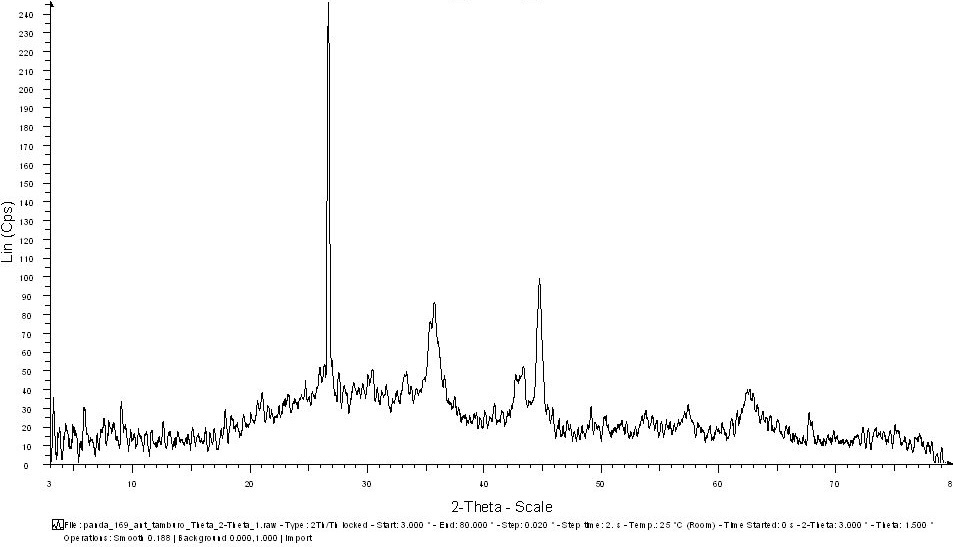
\includegraphics[scale=0.46]{images/panda_169_ant_edit.jpg}
    \caption{PXRD spectrum of Panda Ant sample.}
    \label{fig:Panda_Ant_PXRD}
\end{figure} 

\textbf{Panda Post} \\
The spectrum (Fig.\ref{fig:Panda_Post_PXRD}), in this case, showed some different peaks, but more background. \\
The mineral phases identified were the following:

\setlist{nolistsep}
\begin{enumerate}[noitemsep]
    \item Quartz (JCPDS code: 00-033-1161)
    \item Hematite (JCPDS code: 00-001-1053)
    \item Graphite (JCPDS code: 00-002-0456)
    \item Aluminium Iron Silicon (JCPDS code: 00-045-1205)
    \item Iron (JCPDS code: 00-003-1050)
    \item Magnetite (JCPDS code: 00-019-0629)
    \item Maghemite (JCPDS code: 00-013-0458)
\end{enumerate}

\begin{figure}[H]
\centering
    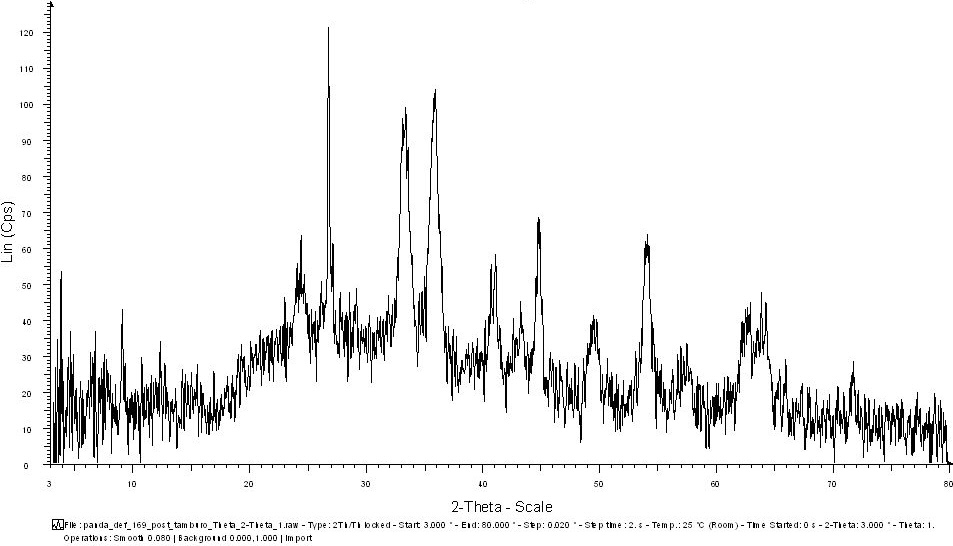
\includegraphics[scale=0.46]{images/panda_169_post_edit.jpg}
    \caption{PXRD spectrum of Panda Post sample.}
    \label{fig:Panda_Post_PXRD}
\end{figure} 

\pagebreak

\textbf{500X Ant} \\
The spectrum (Fig.\ref{fig:500X_Ant_PXRD}) showed some major peaks attributed to:

\setlist{nolistsep}
\begin{enumerate}[noitemsep]
   \item Magnetite (JCPDS code: 00-019-0629)
    \item Maghemite (JCPDS code: 00-004-0755)
    \item Copper Iron Manganese Oxide (JCPDS code: 00-020-0358)
    \item Hematite (JCPDS code: 00-033-0664)
    \item Graphite (JCPDS code:00-002-0456)
    \item Aluminium Iron Silicon (JCPDS code: 00-045-1205)
    \item Goethite (JCPDS code: 00-003-0249)
\end{enumerate}

\begin{figure}[H]
\centering
    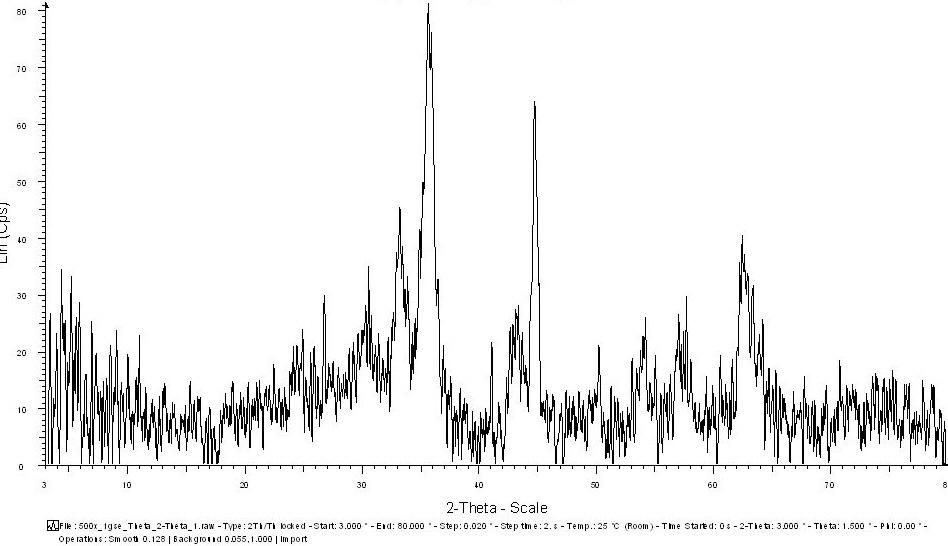
\includegraphics[scale=0.46]{images/500X_1gse_disco_ant_edit.jpg}
    \caption{PXRD spectrum of 500X Ant sample.}
    \label{fig:500X_Ant_PXRD}
\end{figure} 

\textbf{500X Post} \\
The spectrum (Fig.\ref{fig:500X_Post_PXRD}) showed some major peaks attributed to:

\setlist{nolistsep}
\begin{enumerate}[noitemsep]
    \item Magnetite (JCPDS code: 00-001-1111)
    \item Quartz (JCPDS code: 00-033-1161)
    \item Coesite (JCPDS code: 00-014-0654) or Iron Phosphate (JCPDS code: 00-0-14-0147)
    \item Manganese Iron Oxide (JCPDS code: 00-024-0507)
    \item Aluminium Copper Manganese (JCPDS: 00-025-1122) or Sodium Aluminium Oxide (JCPDS: 00-020-1073)
\end{enumerate}

\begin{figure}[H]
\centering
    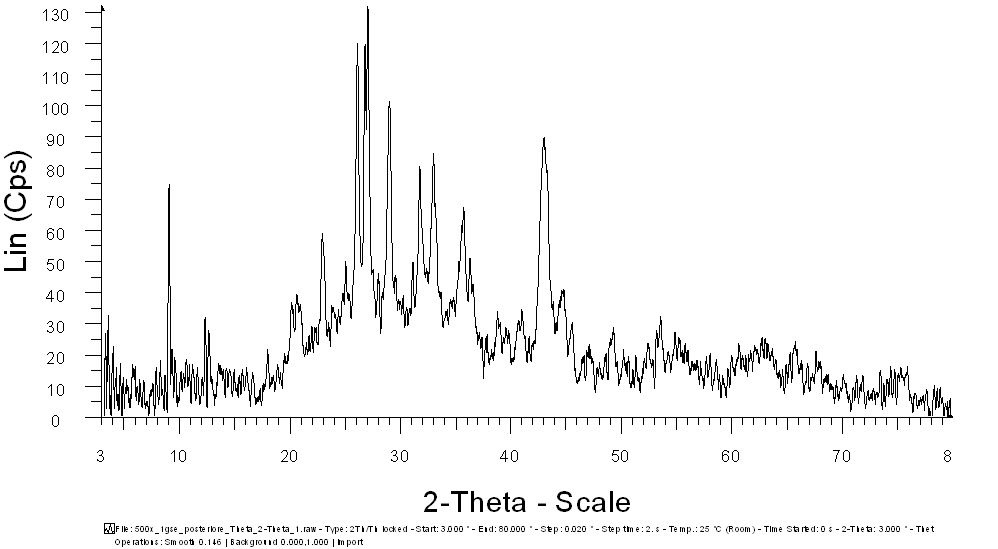
\includegraphics[scale=0.46]{images/500x_post.jpg}
    \caption{PXRD spectrum of 500X Post sample.}
    \label{fig:500X_Post_PXRD}
\end{figure} 

\textbf{500L Ant} \\
The spectrum (Fig.\ref{fig:500L_Ant_PXRD}) showed some major peaks attributed to:

\setlist{nolistsep}
\begin{enumerate}[noitemsep]
    \item Magnetite (JCPDS code: 00-019-0629)
    \item Hematite (JCPDS code: 00-033-0664)
    \item Maghemite (JCPDS code: 00-004-0755)
    \item Allophane (JCPDS code: 00-038-0449)
    \item Graphite (JCPDS code: 00-002-0456)
    \item Goethite (JCPDS code: 00-002-0281)
\end{enumerate}

\begin{figure}[H]
\centering
    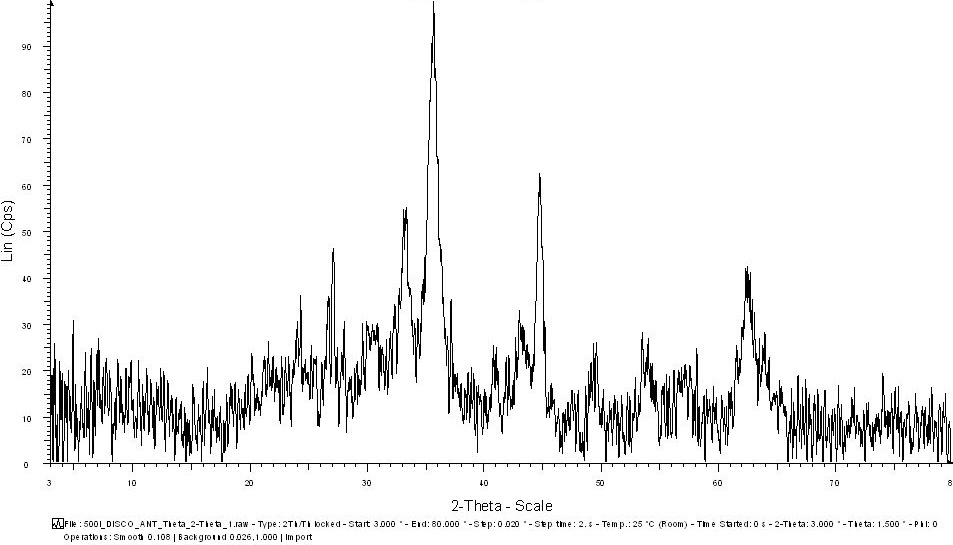
\includegraphics[scale=0.46]{images/500L_DISCO_ANT_edit.jpg}
    \caption{PXRD spectrum of 500L Ant sample.}
    \label{fig:500L_Ant_PXRD}
\end{figure} 

\textbf{500L Post} \\
The spectrum (Fig.\ref{fig:500L_Post_PXRD}) showed some major peaks attributed to:

\setlist{nolistsep}
\begin{enumerate}[noitemsep]
    \item Magnetite (JCPDS code: 00-025-1376)
    \item Hematite (JCPDS code: 00-024-0072)
    \item Maghemite (JCPDS code: 00-004-0755)
    \item Quartz (JCPDS code: 00-001-0649)
    \item Aluminium Iron Silicon (JCPDS: 00-045-1206)
\end{enumerate}

\begin{figure}[H]
\centering
    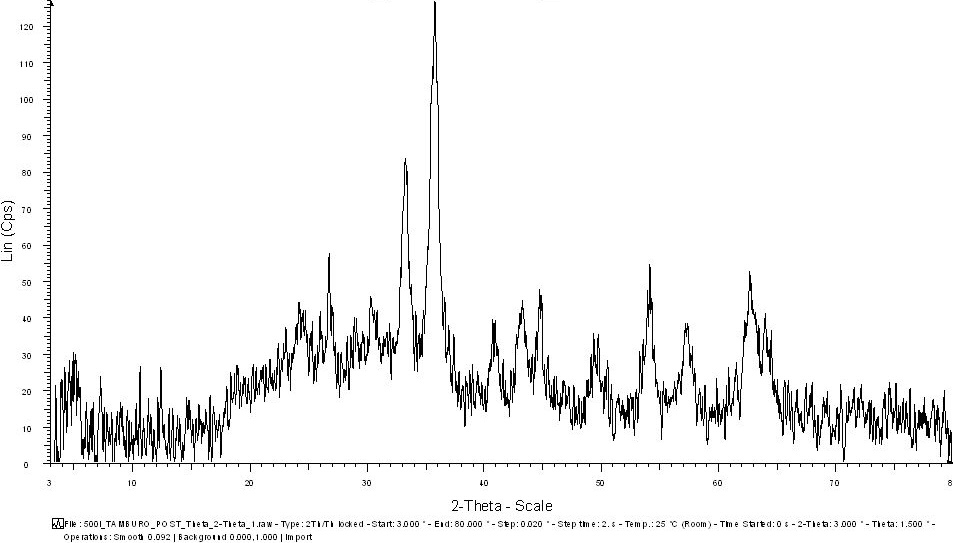
\includegraphics[scale=0.46]{images/500L_tamburo_post_edit.jpg}
    \caption{PXRD spectrum of 500L Post sample.}
    \label{fig:500L_Post_PXRD}
\end{figure} 

\textbf{Ypsilon Ant} \\
The spectrum (Fig.\ref{fig:Ypsilon_Ant_PXRD}) showed some major peaks attributed to:

\setlist{nolistsep}
\begin{enumerate}[noitemsep]
    \item Magnetite (JCPDS code: 00-019-0629)
    \item Hematite (JCPDS code: 00-033-0664)
    \item Maghemite (JCPDS code: 00-004-0755)
    \item Iron (JCPDS code: 00-103-1050)
\end{enumerate}

\begin{figure}[H]
\centering
    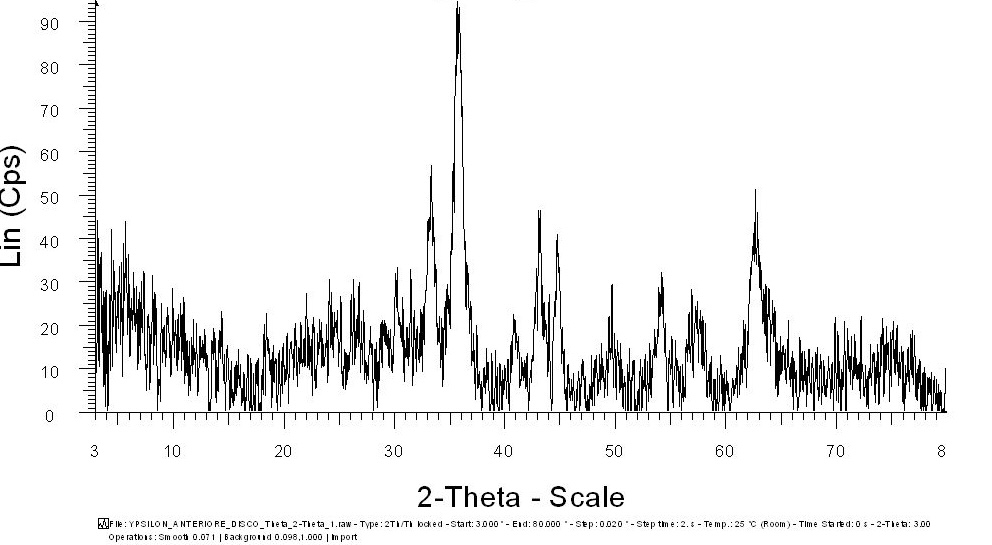
\includegraphics[scale=0.46]{images/YPSILON_ANT_DISCO.jpg}
    \caption{PXRD spectrum of Ypsilon Ant sample.}
    \label{fig:Ypsilon_Ant_PXRD}
\end{figure} 

\textbf{Ypsilon Post} \\
The spectrum (Fig.\ref{fig:Ypsilon_Ant_PXRD}) showed some major peaks attributed to:

\setlist{nolistsep}
\begin{enumerate}[noitemsep]
    \item Magnetite (JCPDS code: 00-025-1376)
    \item Hematite (JCPDS code: 00-033-0664)
    \item Maghemite (JCPDS code: 00-013-0458)
    \item Quartz (JCPDS code: 00-005-0490)
    \item Iron (JCPDS code: 00-006-0696)
\end{enumerate}

\begin{figure}[H]
\centering
    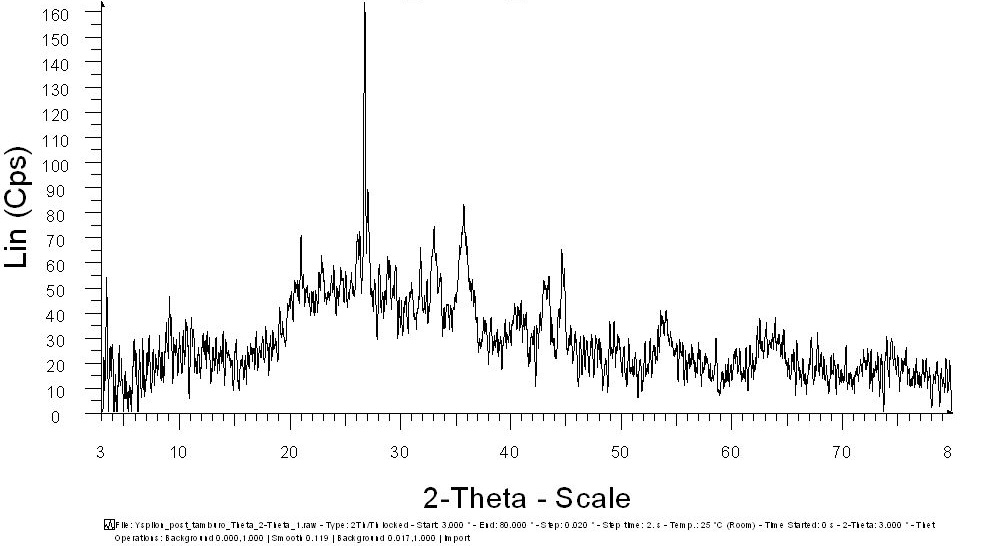
\includegraphics[scale=0.46]{images/YPSILON_POST_TAMBURO.jpg}
    \caption{PXRD spectrum of Ypsilon Post sample.}
    \label{fig:Ypsilon_Post_PXRD}
\end{figure} 

\textbf{Corolla Ant} \\
The spectrum (Fig.\ref{fig:Ypsilon_Ant_PXRD}) showed some major peaks attributed to:

\setlist{nolistsep}
\begin{enumerate}[noitemsep]
    \item Magnetite (JCPDS code: 00-025-1402)
    \item Aluminium Iron Silicon (JCPDS code: 00-045-1205)
    \item Maghemite (JCPDS code: 00-025-1402)
    \item Quartz (JCPDS code: 00-005-0490)
    \item Copper Magnesium Tin (JCPDS code: 00-034-1092) or Copper Tin (JCPDS code: 00-031-0485)
\end{enumerate}

\begin{figure}[H]
\centering
    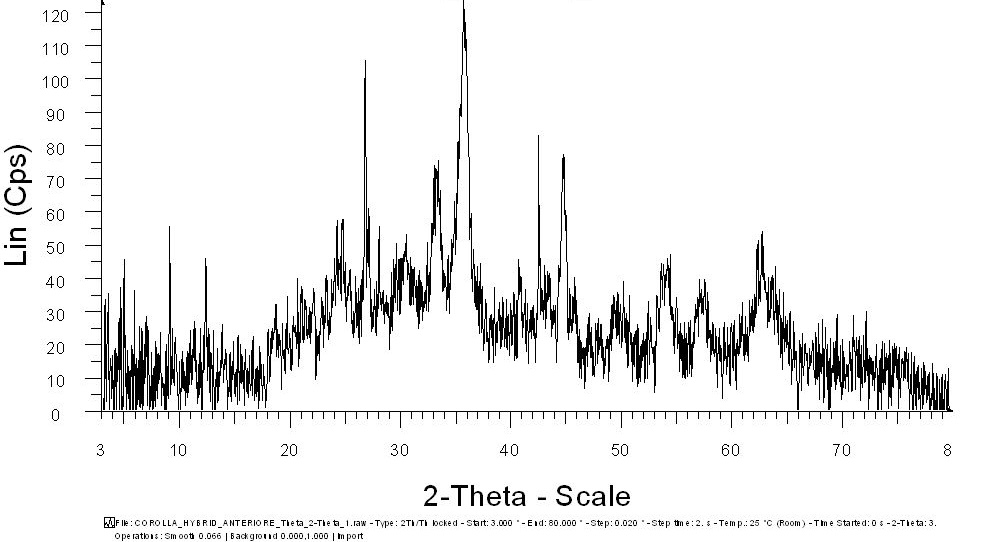
\includegraphics[scale=0.46]{images/Corolla_Hybrid_Ant.jpg}
    \caption{PXRD spectrum of Corolla Ant sample.}
    \label{fig:Corolla_Ant_PXRD}
\end{figure} 
\pagebreak

\section{SEM-EDX Before Interaction}

\subsection{Dimensional Analyses}

For each sample a histogram was created using the "Feret" values obtained with "ImageJ".\\
On the x-axis, the particle diameters corresponding to the "Feret" values were plotted, and on the y-axis, the number of particles with the corresponding diameters was reported. \\
Two red lines were added to each histogram to delineate the diameter values of interest, specifically those under 10 µm, between 10 µm and 2.5 µm, and below 2.5 µm.\\
The resulting histograms were the following:

\begin{figure}[H]
\centering
\begin{subfigure}{.5\textwidth}
  \centering
  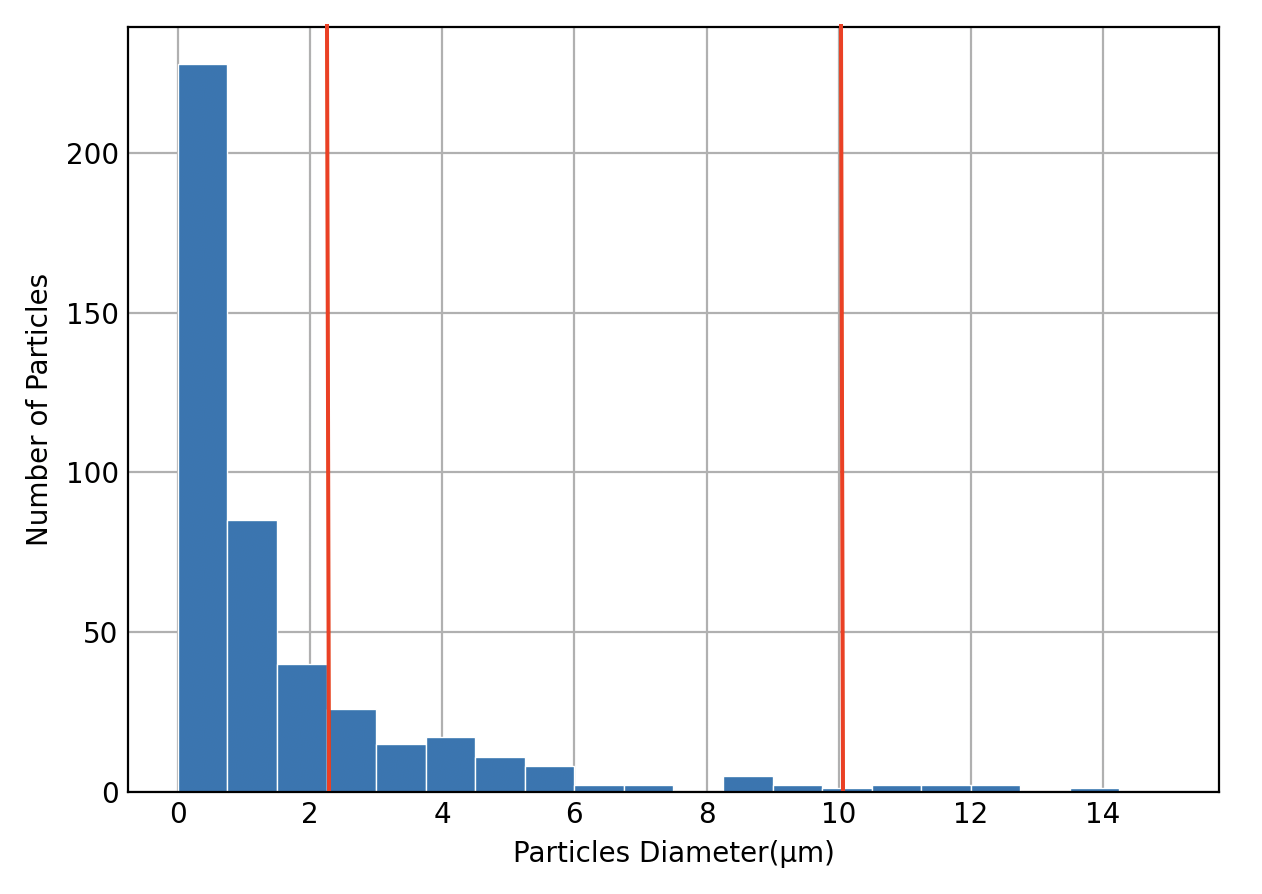
\includegraphics[width=1\linewidth]{images/Panda_Ant_D.png}
  \caption{Panda Ant}
  \label{fig:pandaant}
\end{subfigure}%
\begin{subfigure}{.5\textwidth}
  \centering
  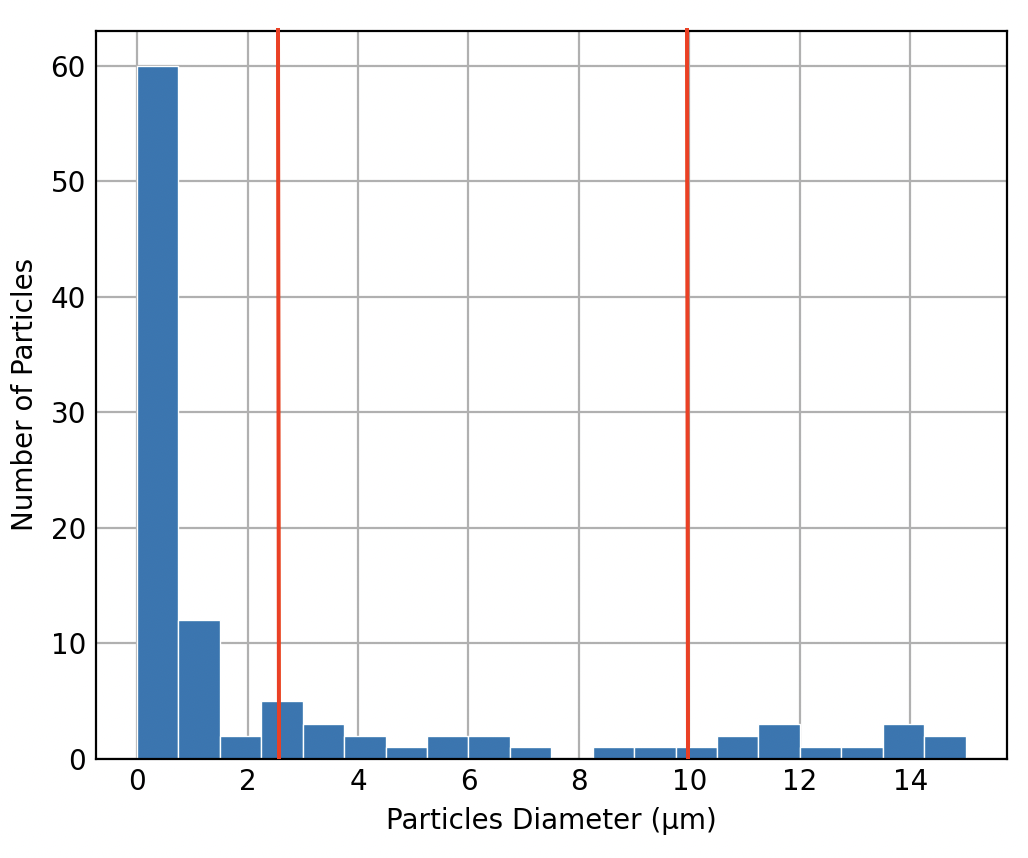
\includegraphics[width=0.85\linewidth]{images/Panda_Post_D.png}
  \caption{Panda Post}
  \label{fig:pandapost}
\end{subfigure}
\caption{Diameter distribution histograms of Panda sample}
\label{fig:1}
\end{figure}

\begin{figure}[H]
\centering
\begin{subfigure}{.5\textwidth}
  \centering
  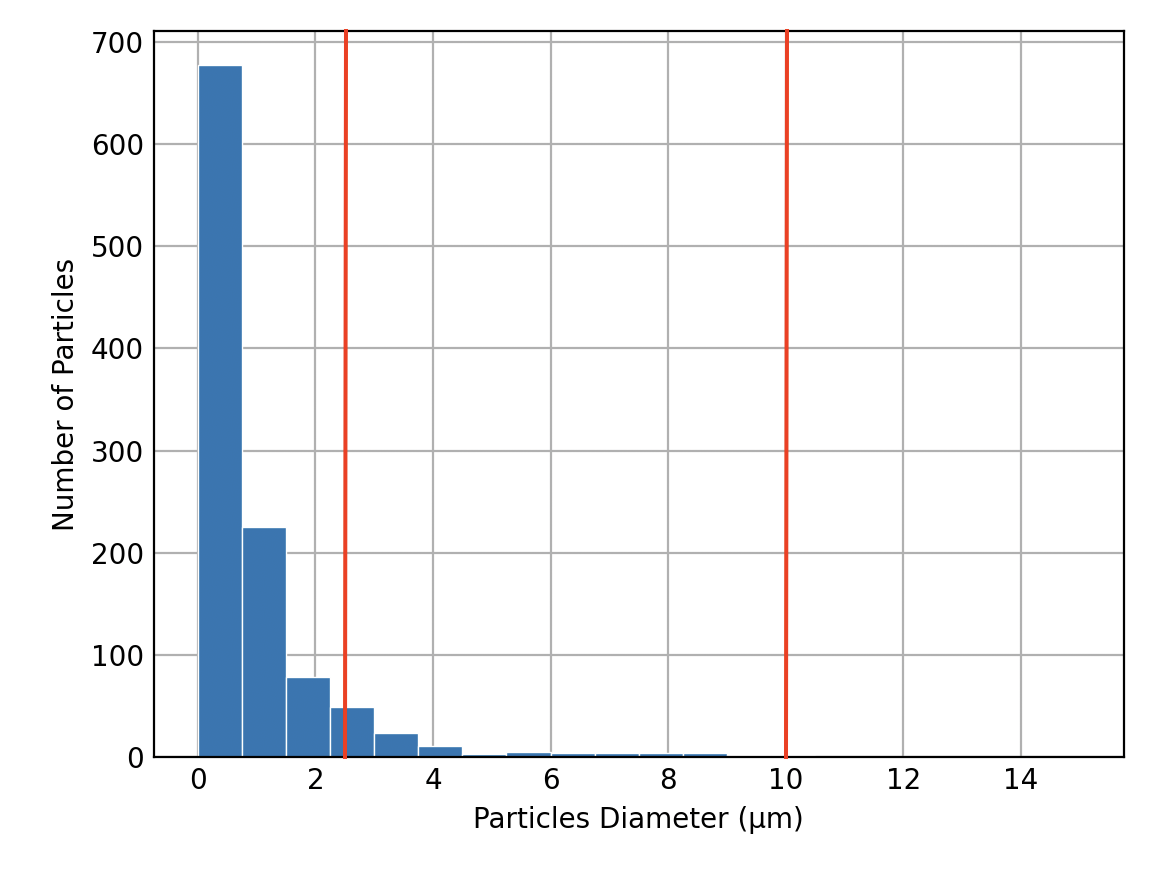
\includegraphics[width=1\linewidth]{images/500X_ant_dis.png}
  \caption{500X Ant}
  \label{fig:500xant}
\end{subfigure}%
\begin{subfigure}{.5\textwidth}
  \centering
  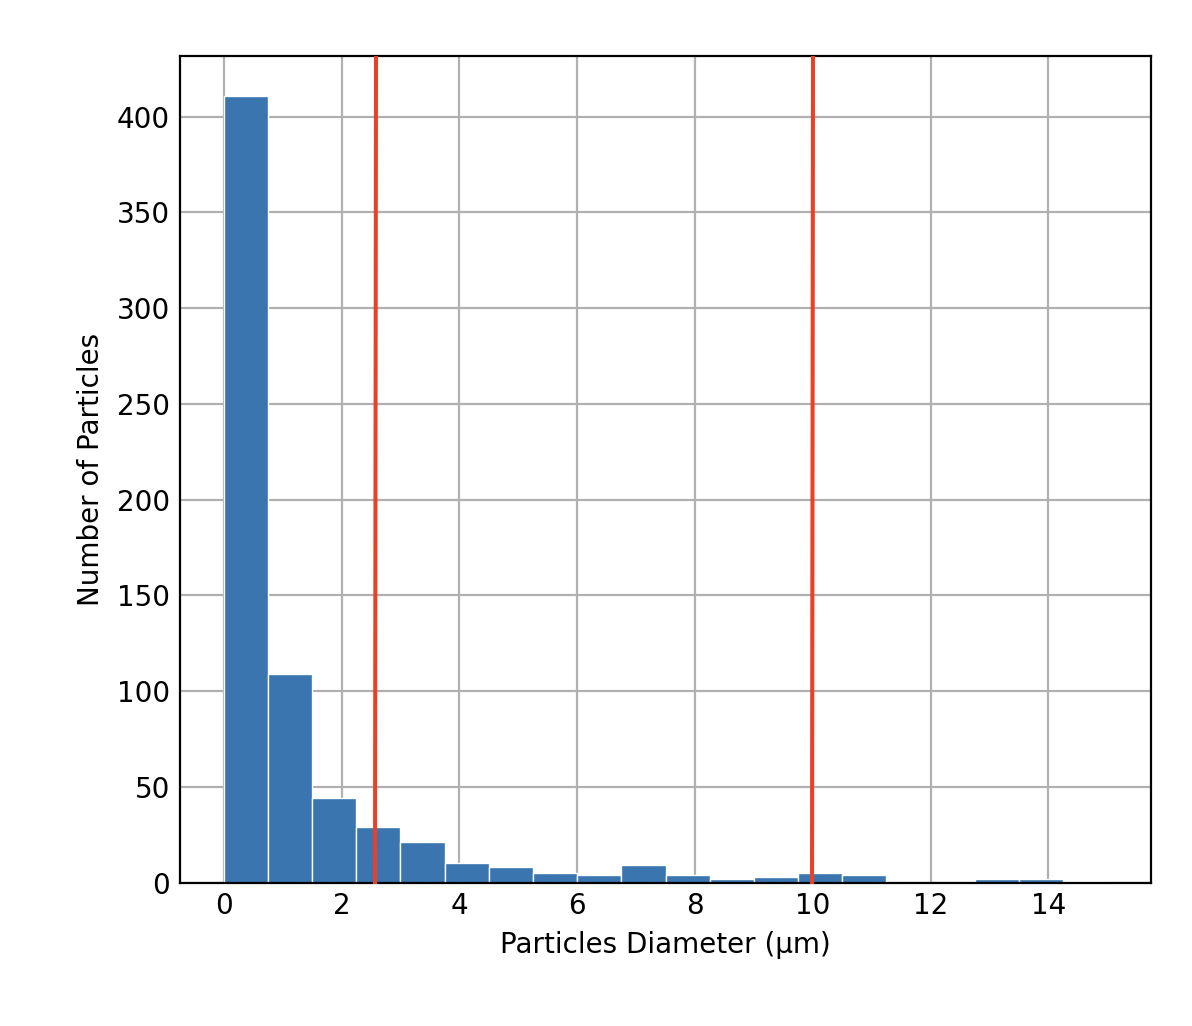
\includegraphics[width=0.9\linewidth]{images/500X_post_dis.png}
  \caption{500X Post}
  \label{fig:500xpost}
\end{subfigure}
\caption{Diameter distribution histograms of 500X sample}
\label{fig:2}
\end{figure}

\begin{figure}[H]
\centering
\begin{subfigure}{.5\textwidth}
  \centering
  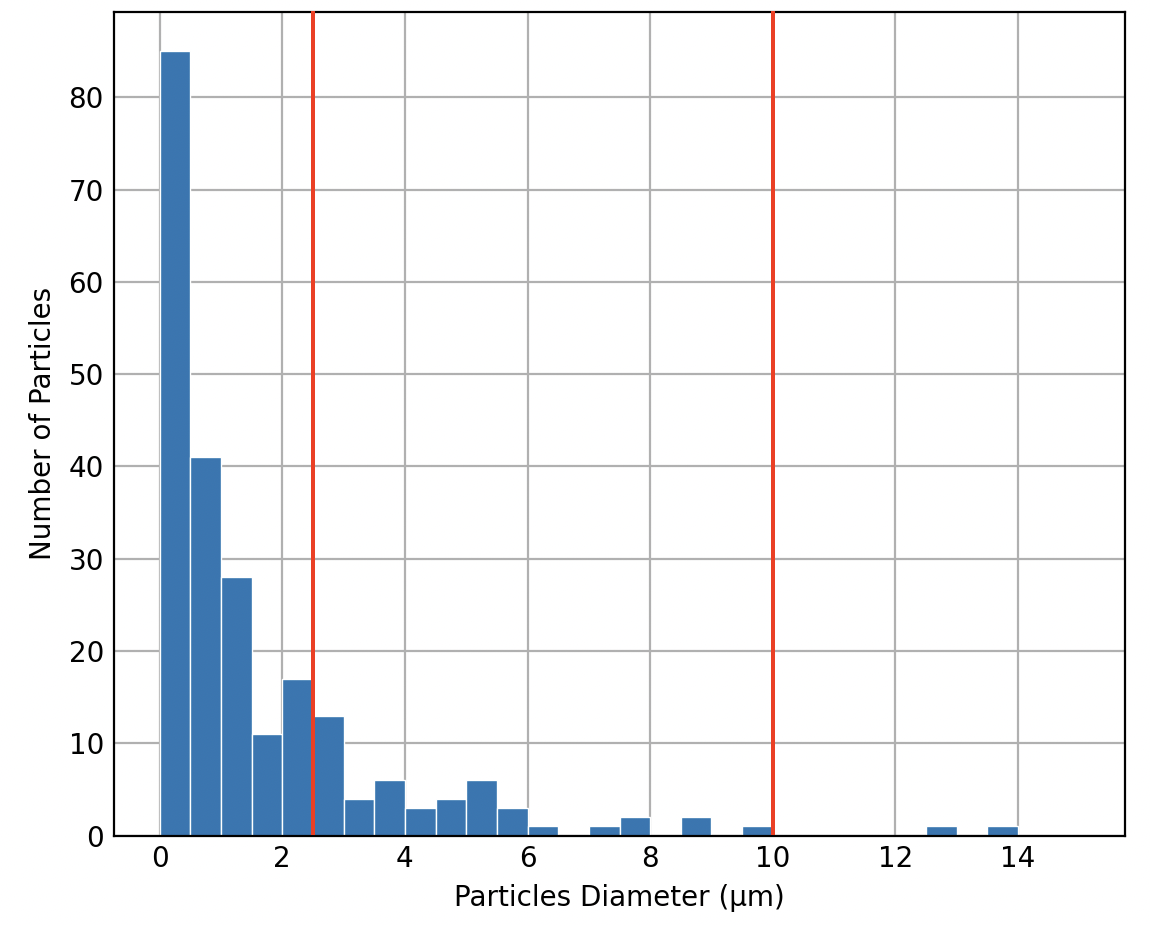
\includegraphics[width=0.85\linewidth]{images/500L_Ant_D.png}
  \caption{500L Ant}
  \label{fig:500lant}
\end{subfigure}%
\begin{subfigure}{.5\textwidth}
  \centering
  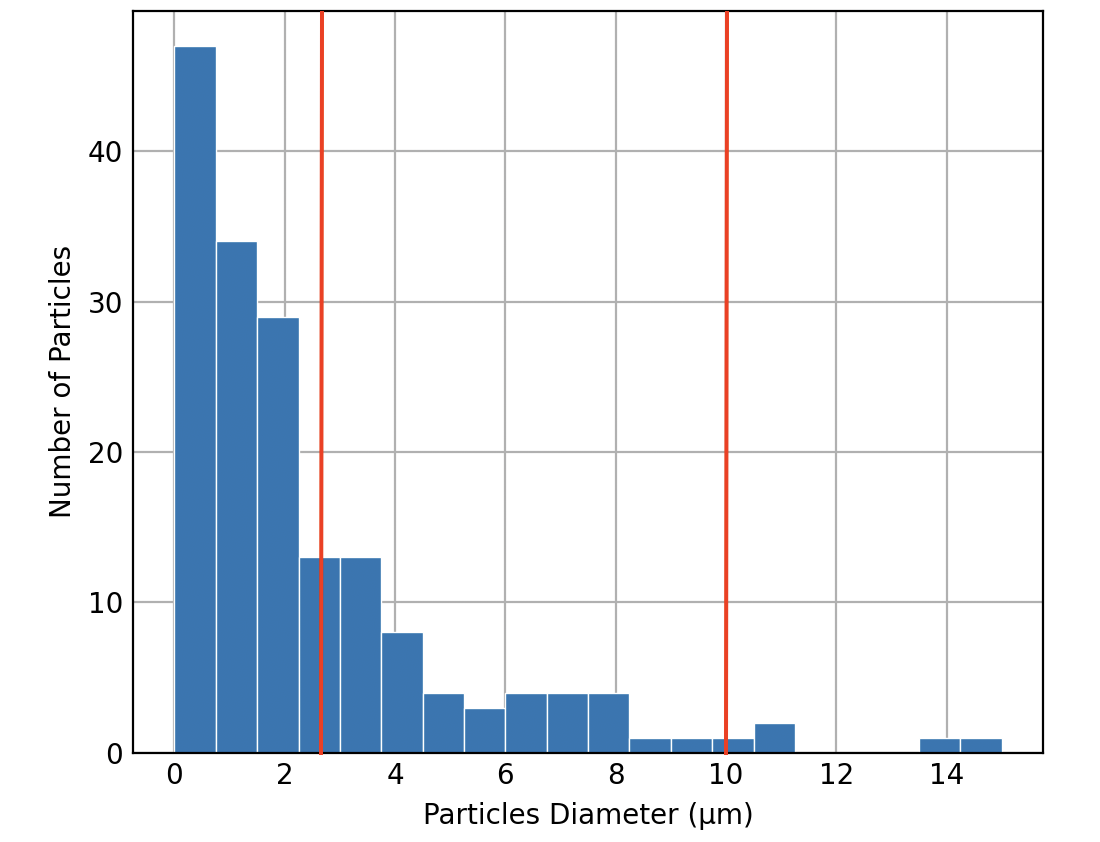
\includegraphics[width=0.9\linewidth]{images/500L_Post_D.png}
  \caption{500L Post}
  \label{fig:500lpost}
\end{subfigure}
\caption{Diameter distribution histograms of 500L sample}
\label{fig:3}
\end{figure}

\begin{figure}[H]
\centering
\begin{subfigure}{.5\textwidth}
  \centering
  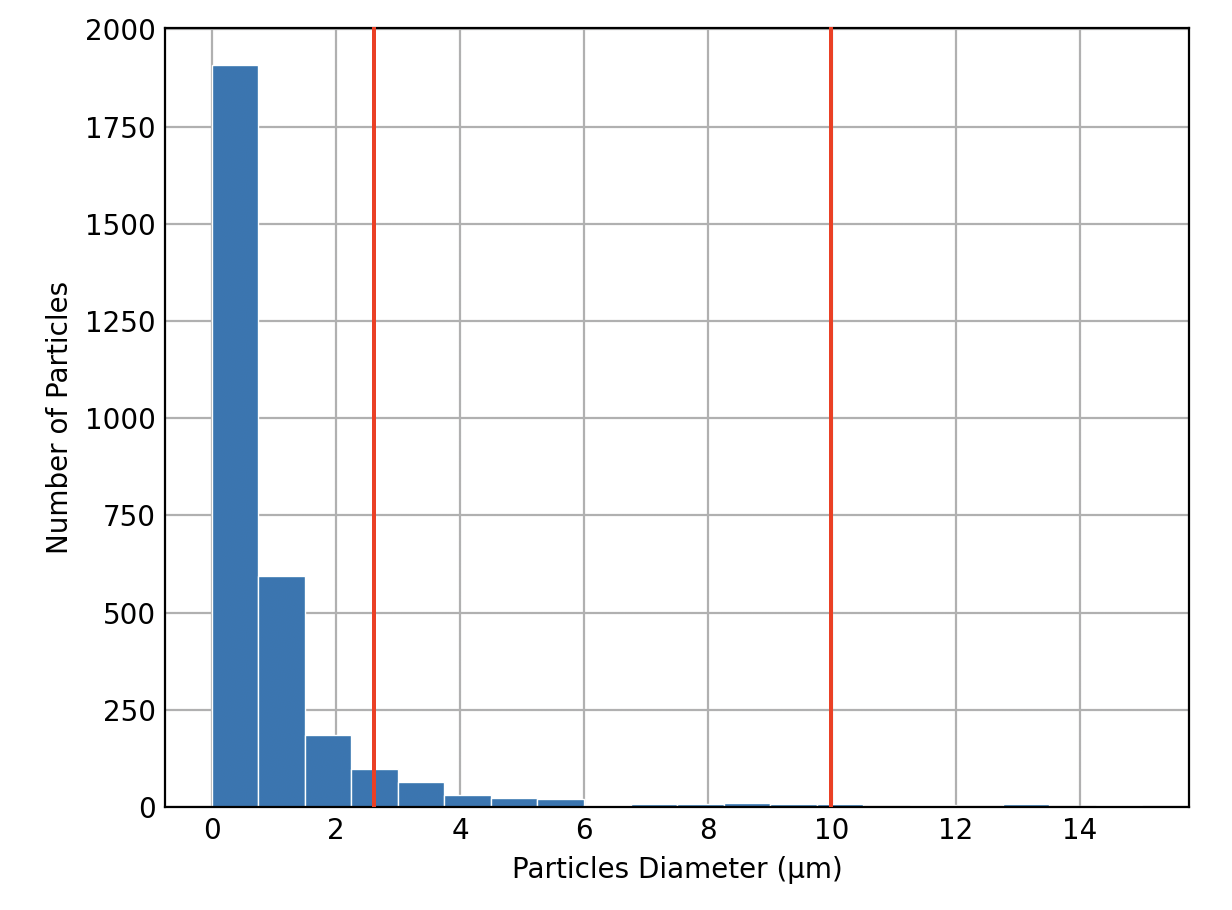
\includegraphics[width=1\linewidth]{images/Ypsilon_Ant_D.png}
  \caption{Ypsilon Ant}
  \label{fig:ypsilonant}
\end{subfigure}%
\begin{subfigure}{.5\textwidth}
  \centering
  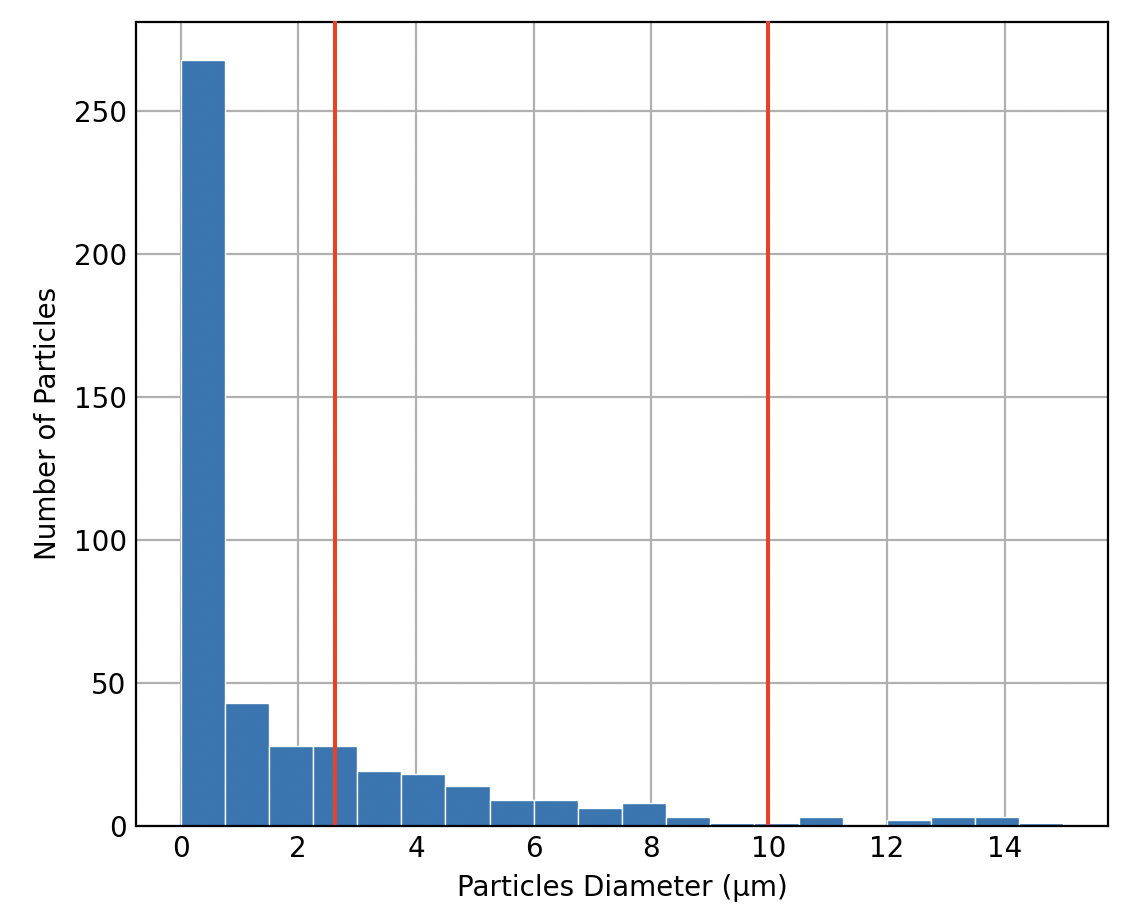
\includegraphics[width=0.9\linewidth]{images/Ypsilon_Post_D.png}
  \caption{Ypsilon Post}
  \label{fig:ypsilonpost}
\end{subfigure}
\caption{Diameter distribution histograms of Ypsilon sample}
\label{fig:4}
\end{figure}

\begin{figure}[H]
\centering
\begin{subfigure}{.5\textwidth}
  \centering
  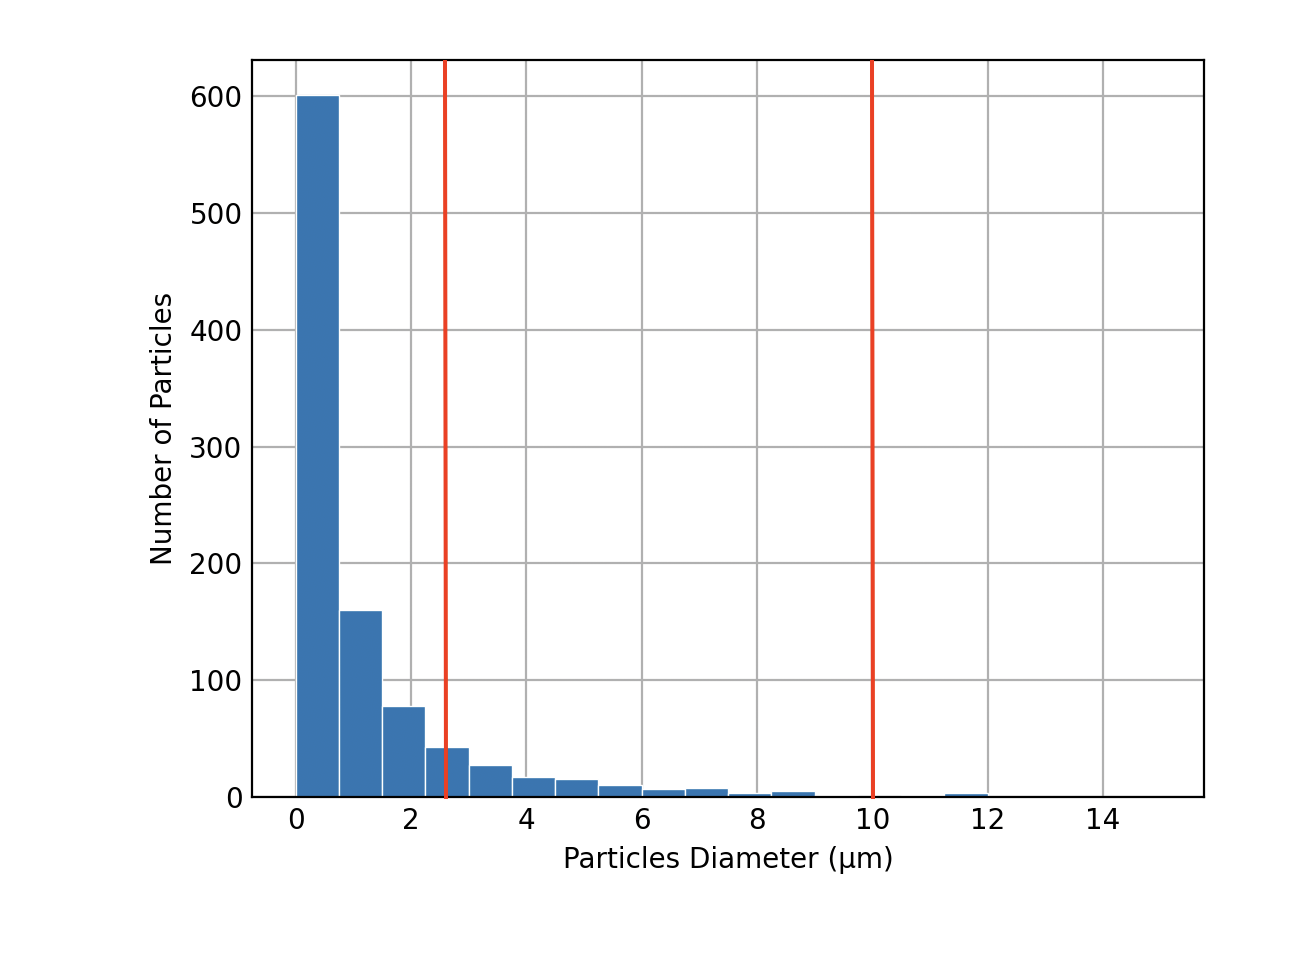
\includegraphics[width=1\linewidth]{images/corolla_ant_dis.png}
  \caption{Corolla Ant}
  \label{fig:corollaant}
\end{subfigure}%
\begin{subfigure}{.5\textwidth}
  \centering
  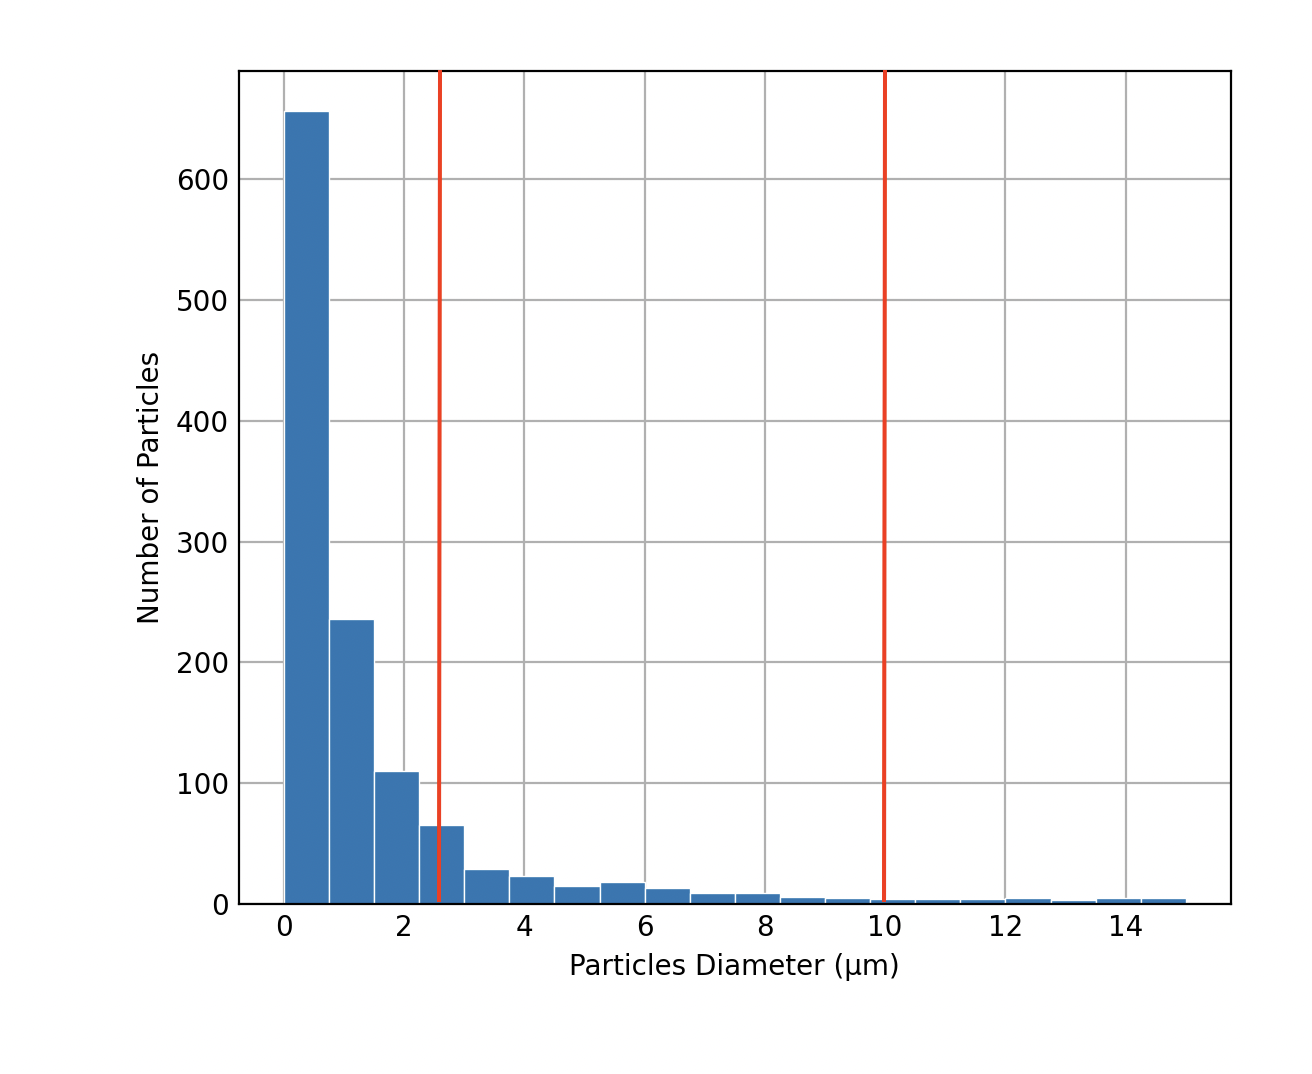
\includegraphics[width=0.9\linewidth]{images/corolla_post_dis.png}
  \caption{Corolla Post}
  \label{fig:corollapost}
\end{subfigure}
\caption{Diameter distribution histograms of Corolla sample}
\label{fig:5}
\end{figure}


The number of total particles identified in each sample was different and to ensure comparability among them, the values obtained from the measurements were transformed into percentages. This approach allowed for a uniform evaluation of the differences between the samples. \\
The percentages, shown in Table \ref{tab:percentages}, refer to the different samples and the particles (p) within the illustrated range of diameter. 

\begin{table}[h]
\centering

\begin{tabular}{l r r r r r}
\hline

Sample & $p \leq 2.5 \mu m$ & $ 2.5 \mu m < p \leq 10 \mu m$ & $p \leq 10 \mu m$ \\

\hline

Panda\_Ant & $80\%$ & $18\%$ & $2\%$ \\
Panda\_Post & $66\%$ & $13\%$ & $21\%$ \\
500X\_Ant & $90\%$ & $9\%$ & $1\%$ \\
500X\_Post & $85\%$ & $12\%$ & $3\%$ \\
500L\_Ant & $79\%$ & $20\%$ & $1\%$ \\
500L\_Post & $66\%$ & $30\%$ & $4\%$ \\
Ypsilon\_Ant & $88\%$ & $8\%$ & $4\%$ \\
Ypsilon\_Post & $72\%$ & $22\%$ & $6\%$ \\
Corolla\_Ant & $87\%$ & $12\%$ & $1\%$ \\
Corolla\_Post & $83\%$ & $12\%$ & $4\%$ \\

        \hline

    \end{tabular}
     \caption{Percentages of particles (p) found in the different samples with focus on the diameters of interest. }
     \label{tab:percentages}
\end{table}

\subsection{Heavy Metals Content}

A grouped bar chart was generated using the results obtained from EDX analysis to compare the presence of various heavy metals in each sample. \\
The x-axis denotes the sample, while the y-axis indicates the frequency, out of 100 occurrences per sample, of each specific heavy metal detected.


\begin{figure}[H]
\centering
    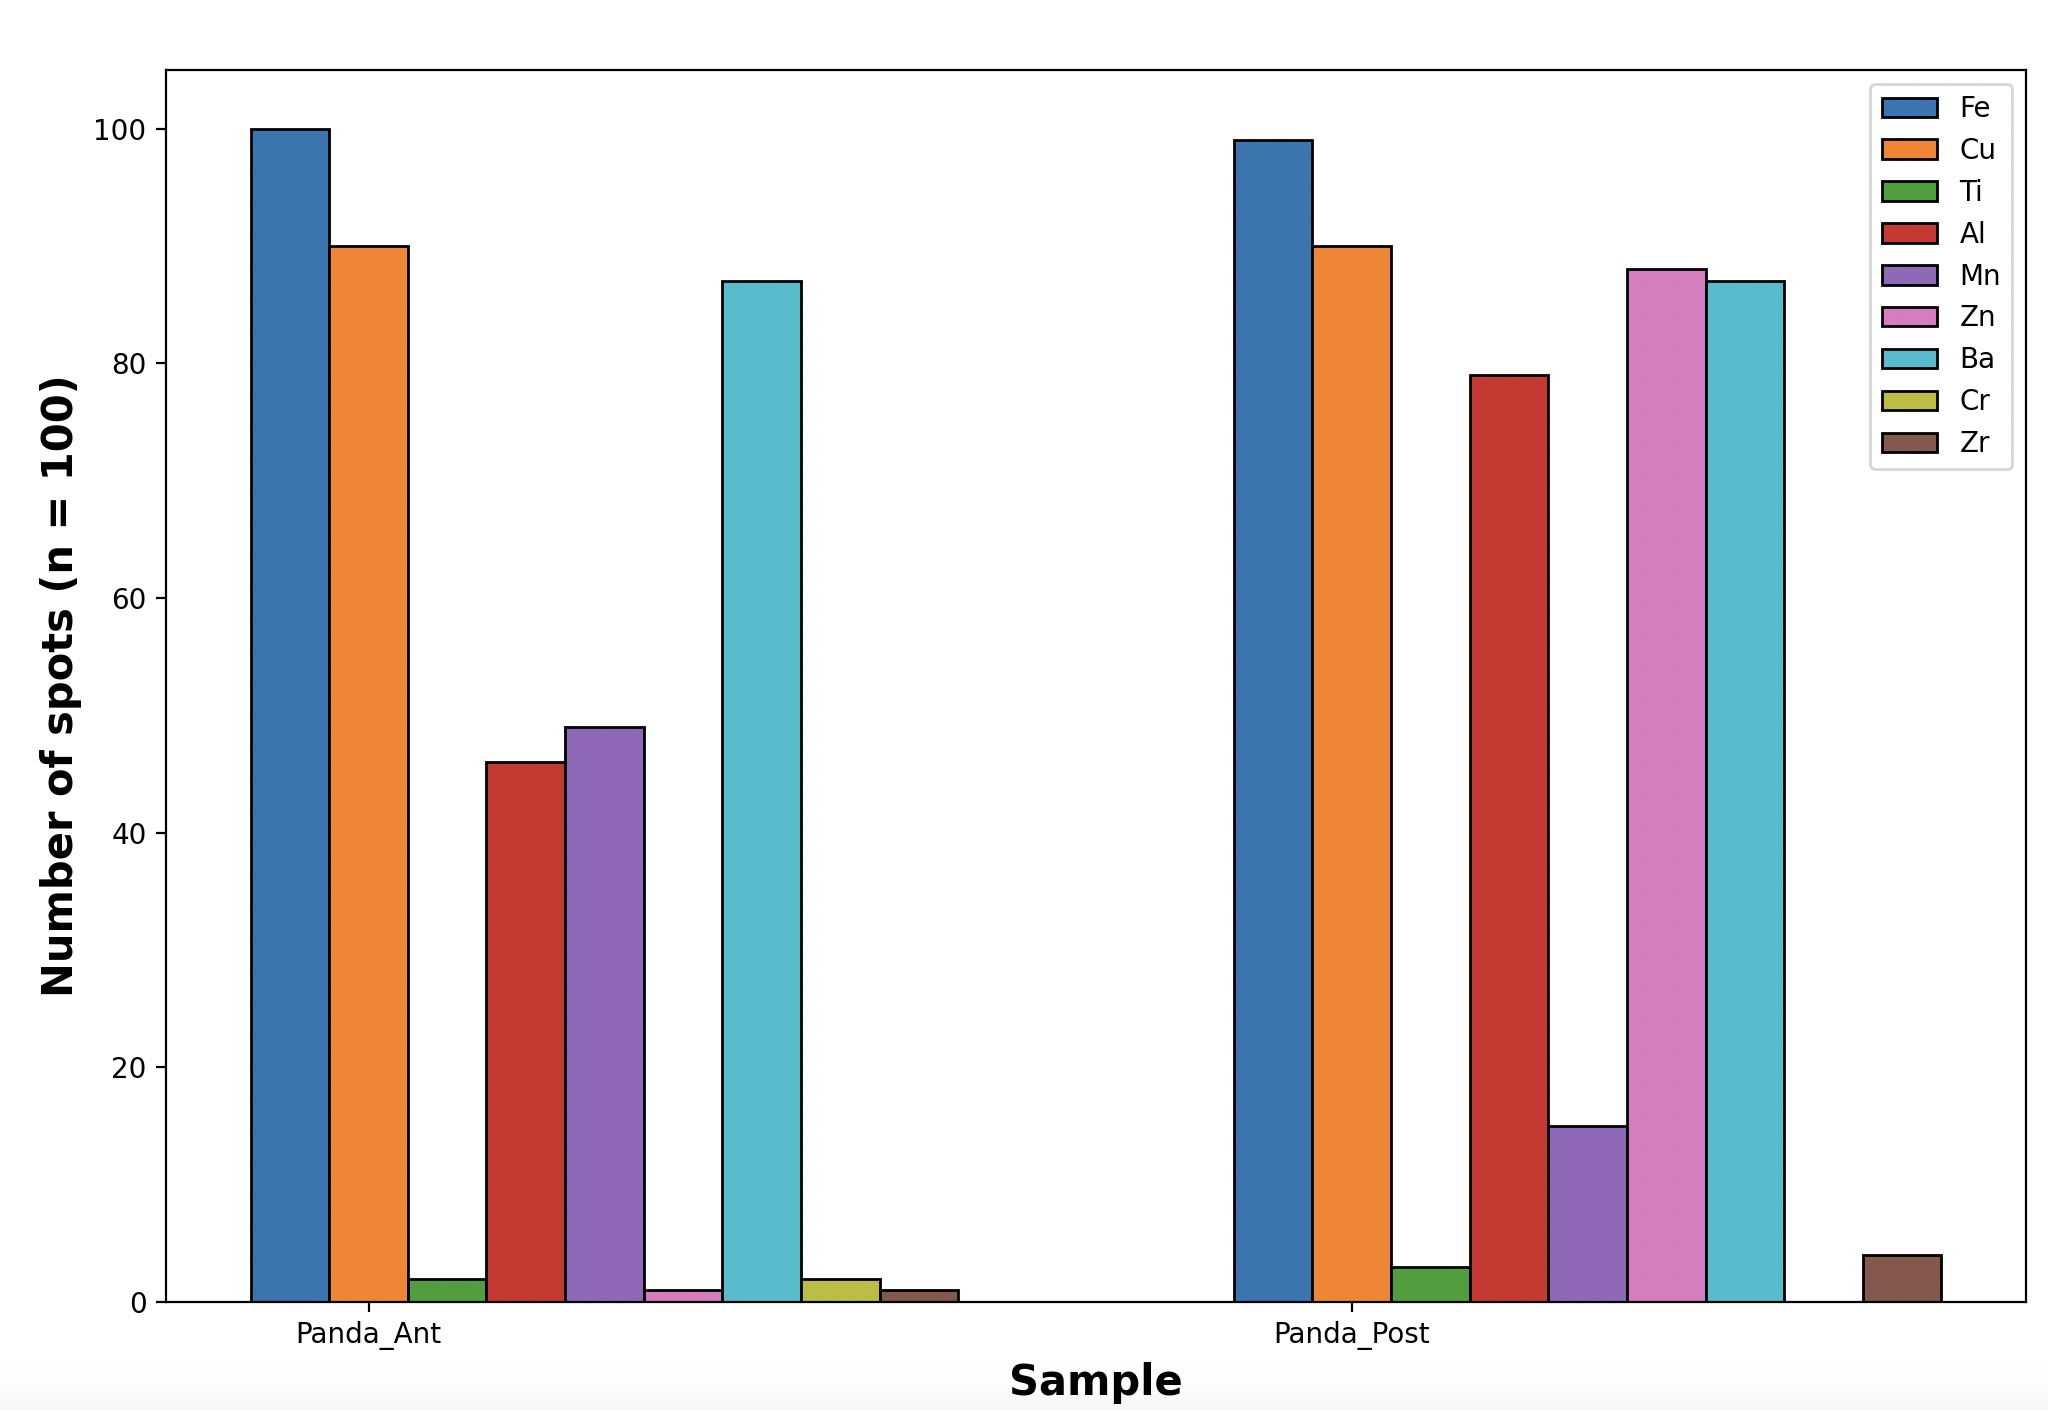
\includegraphics[scale=0.27]{images/Panda_HM.png}
    \caption{Grouped bar chart of Panda sample.}
    \label{fig:Panda_HM}
\end{figure} 

\begin{figure}[H]
\centering
    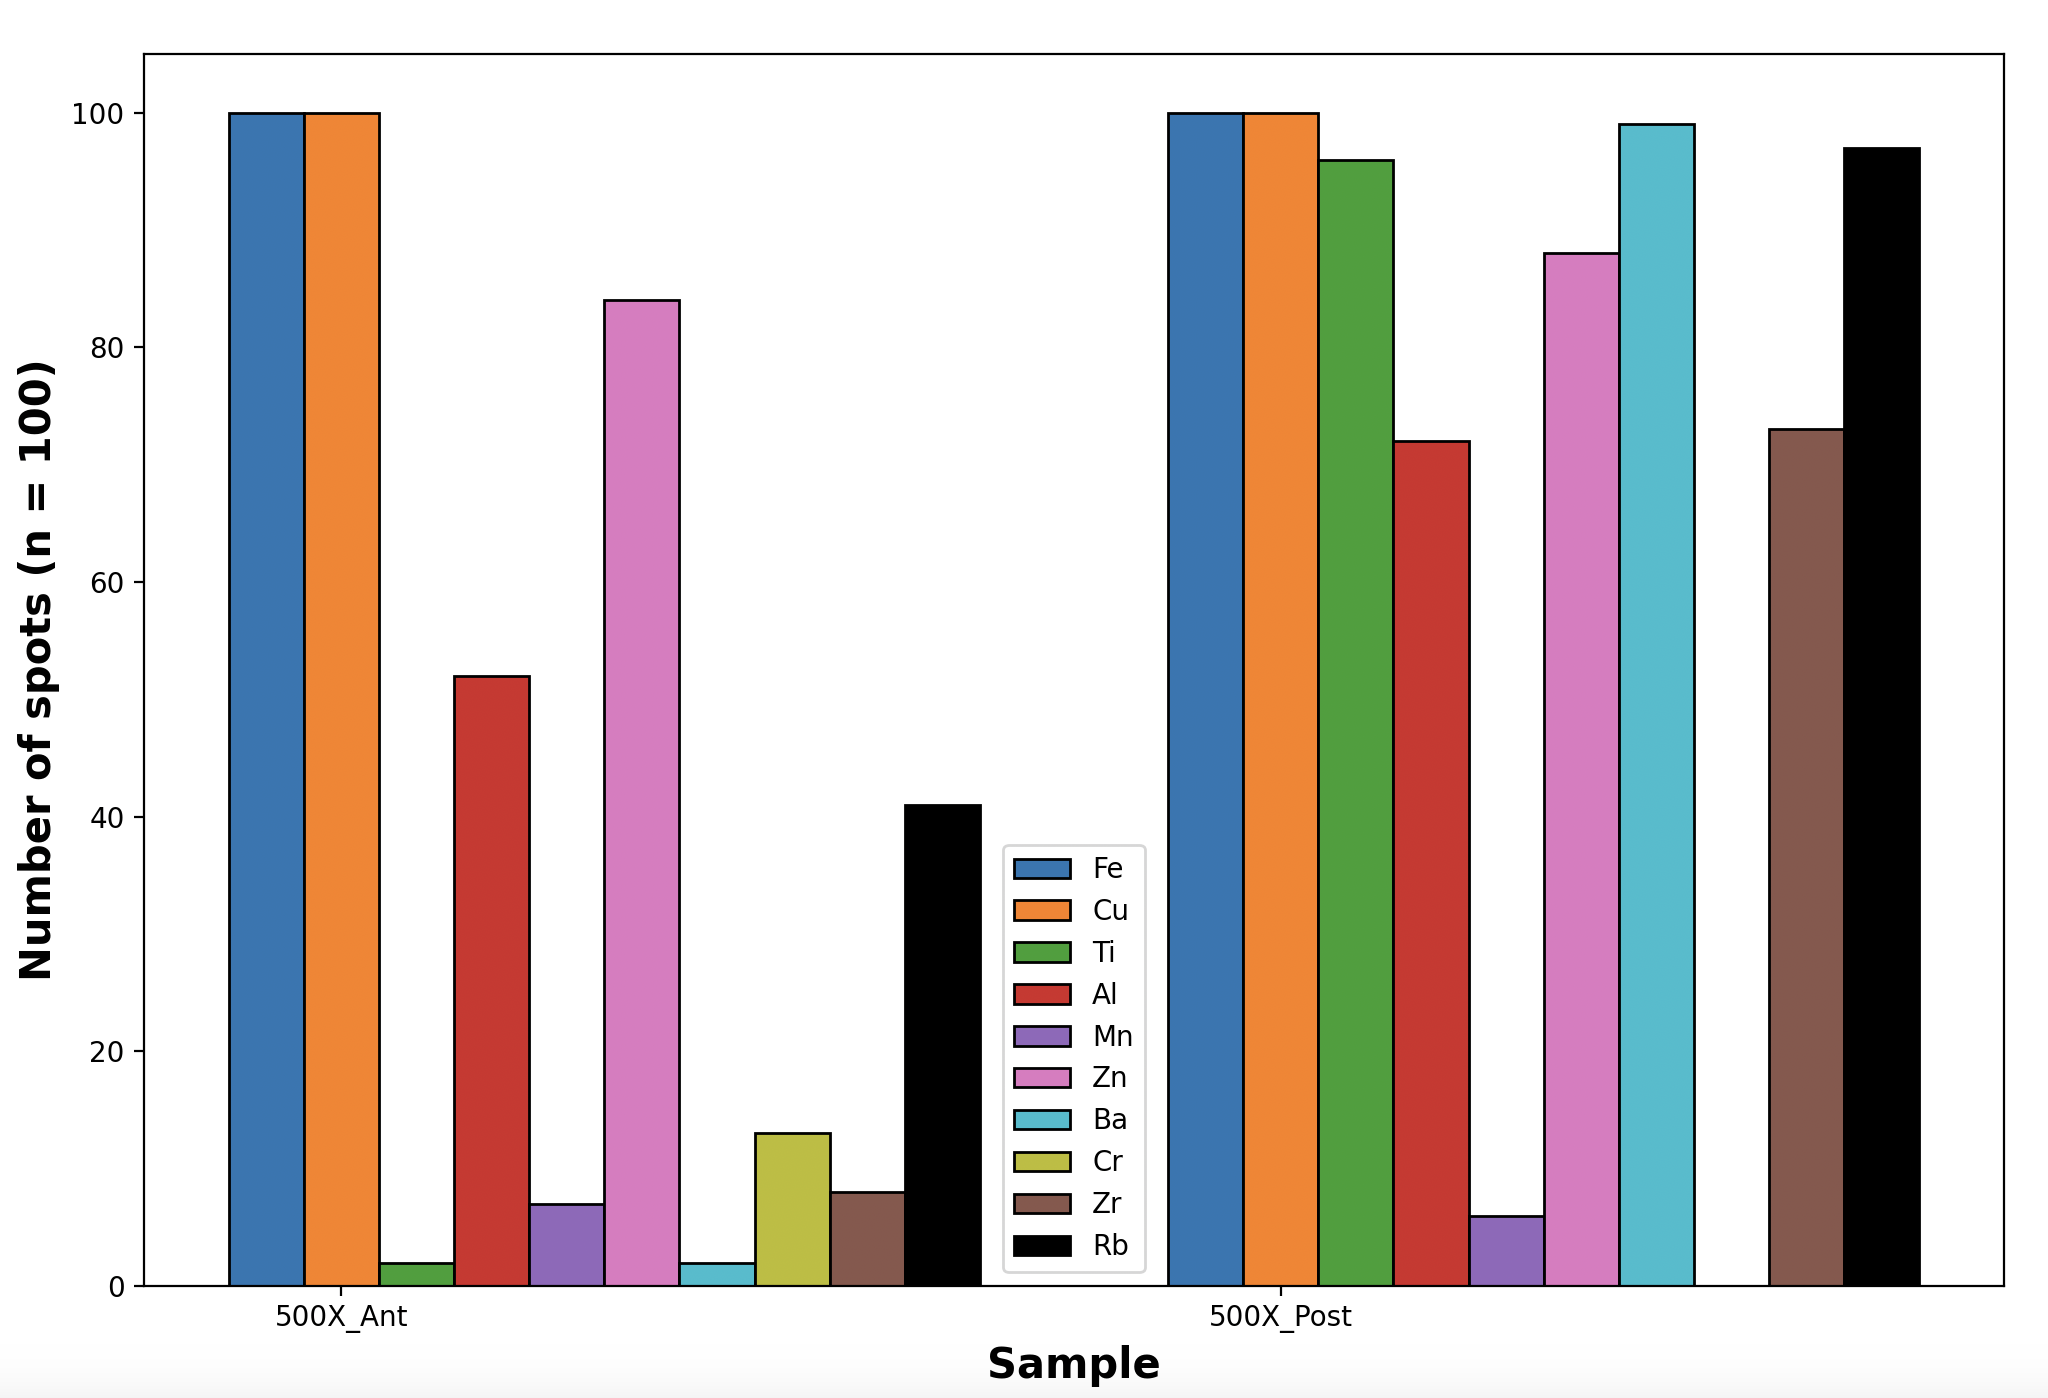
\includegraphics[scale=0.27]{images/500X_HM.png}
    \caption{Grouped bar chart of 500X sample.}
    \label{fig:500X_HM}
\end{figure} 

\begin{figure}[H]
\centering
    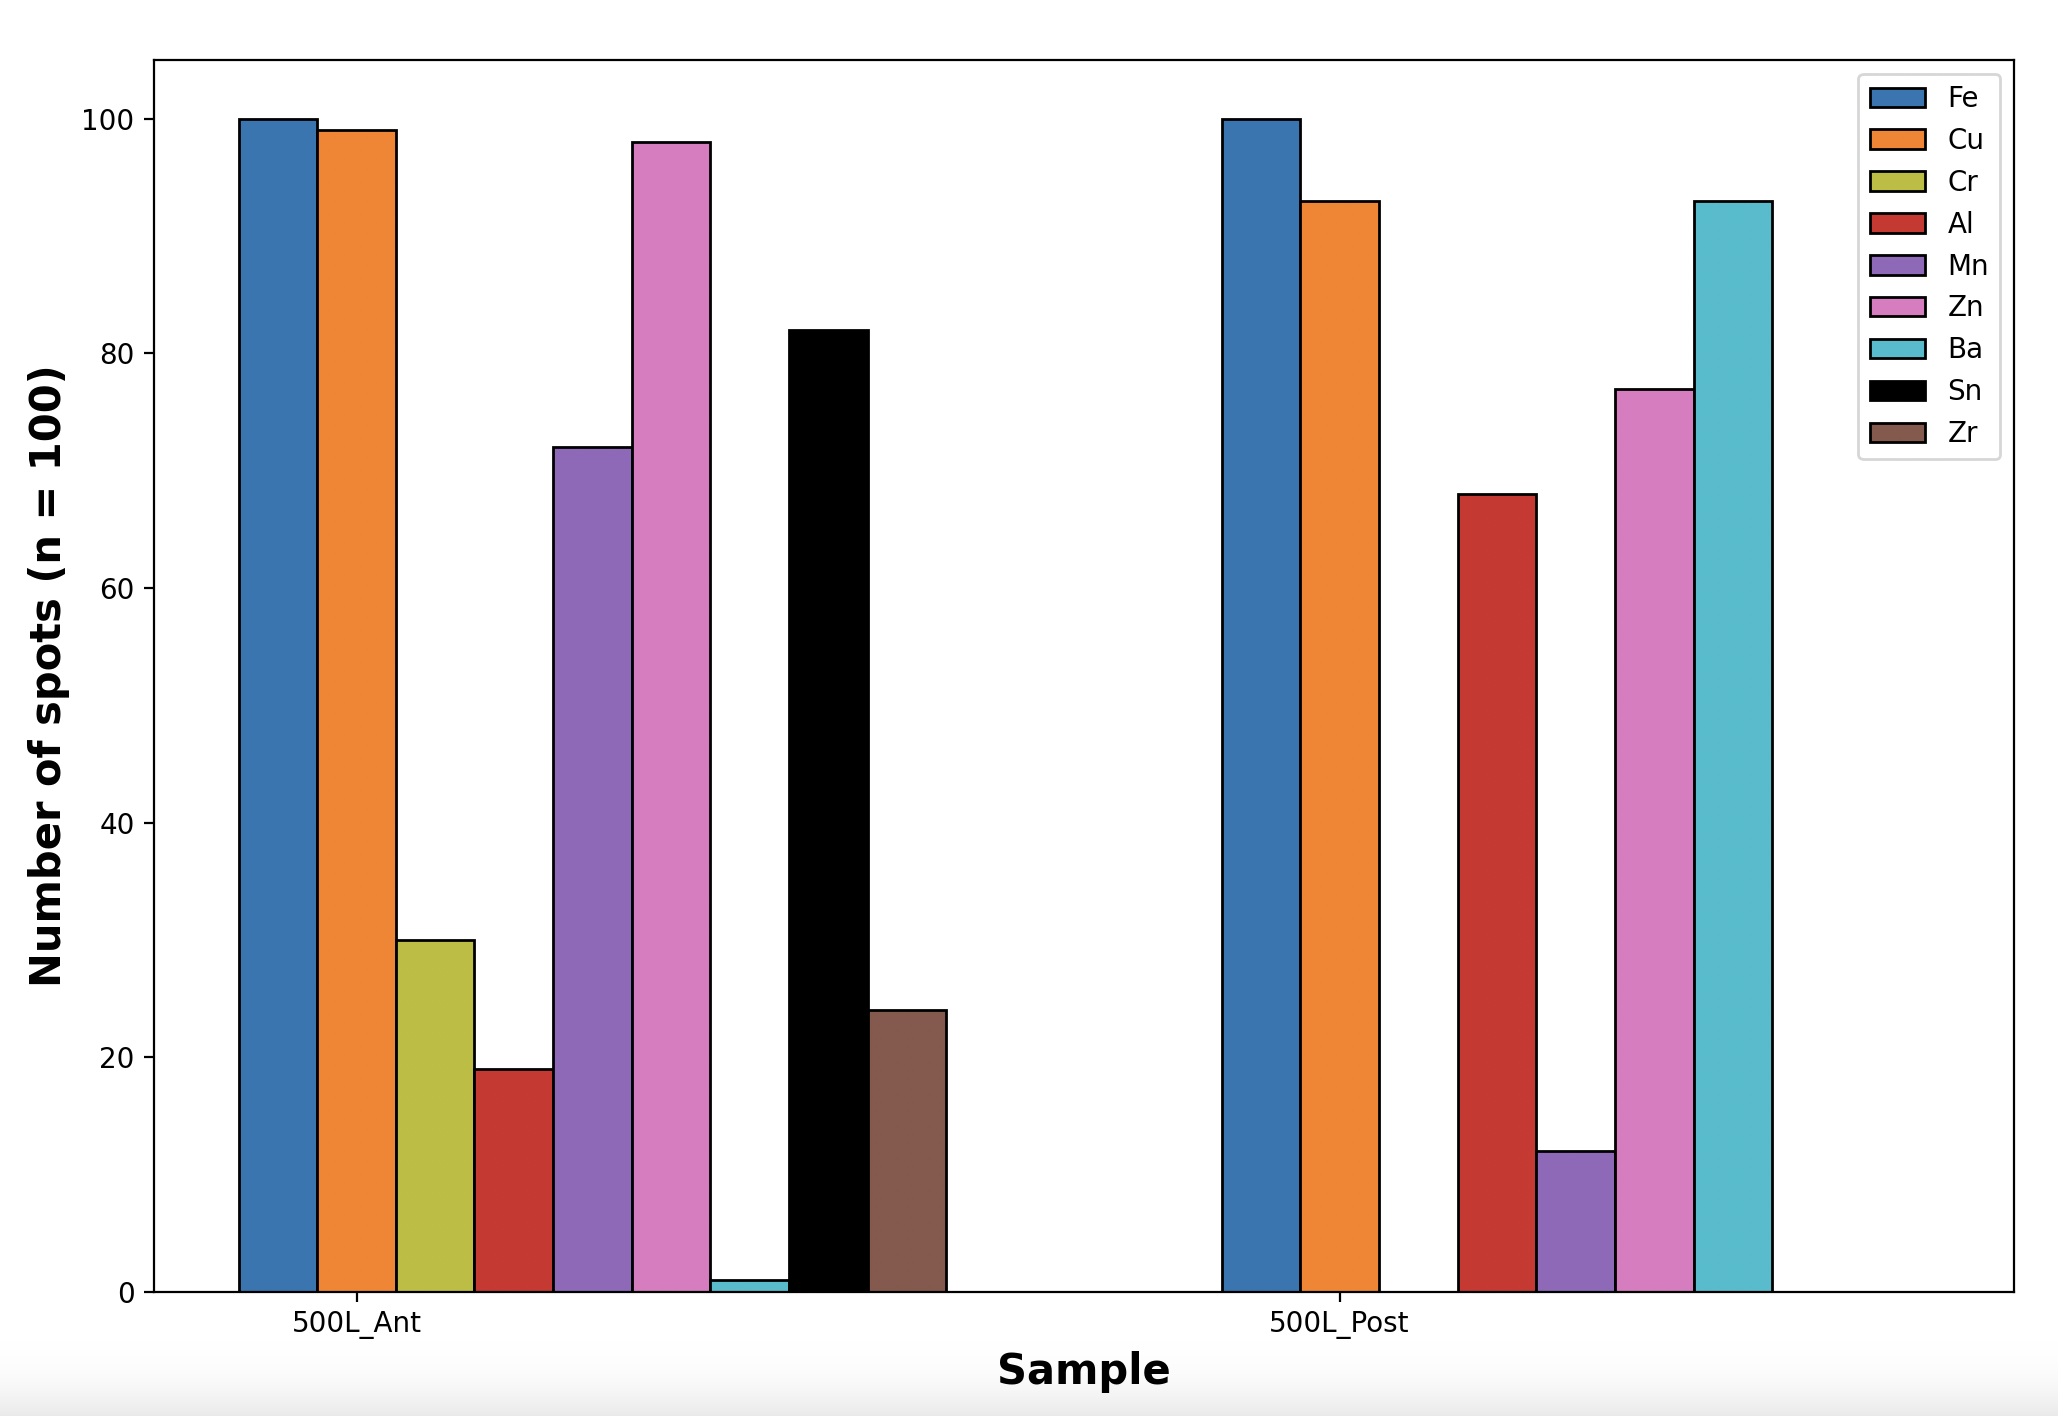
\includegraphics[scale=0.27]{images/500L_HM.png}
    \caption{Grouped bar chart of 500L sample.}
    \label{fig:500L_HM}
\end{figure} 

\begin{figure}[H]
\centering
    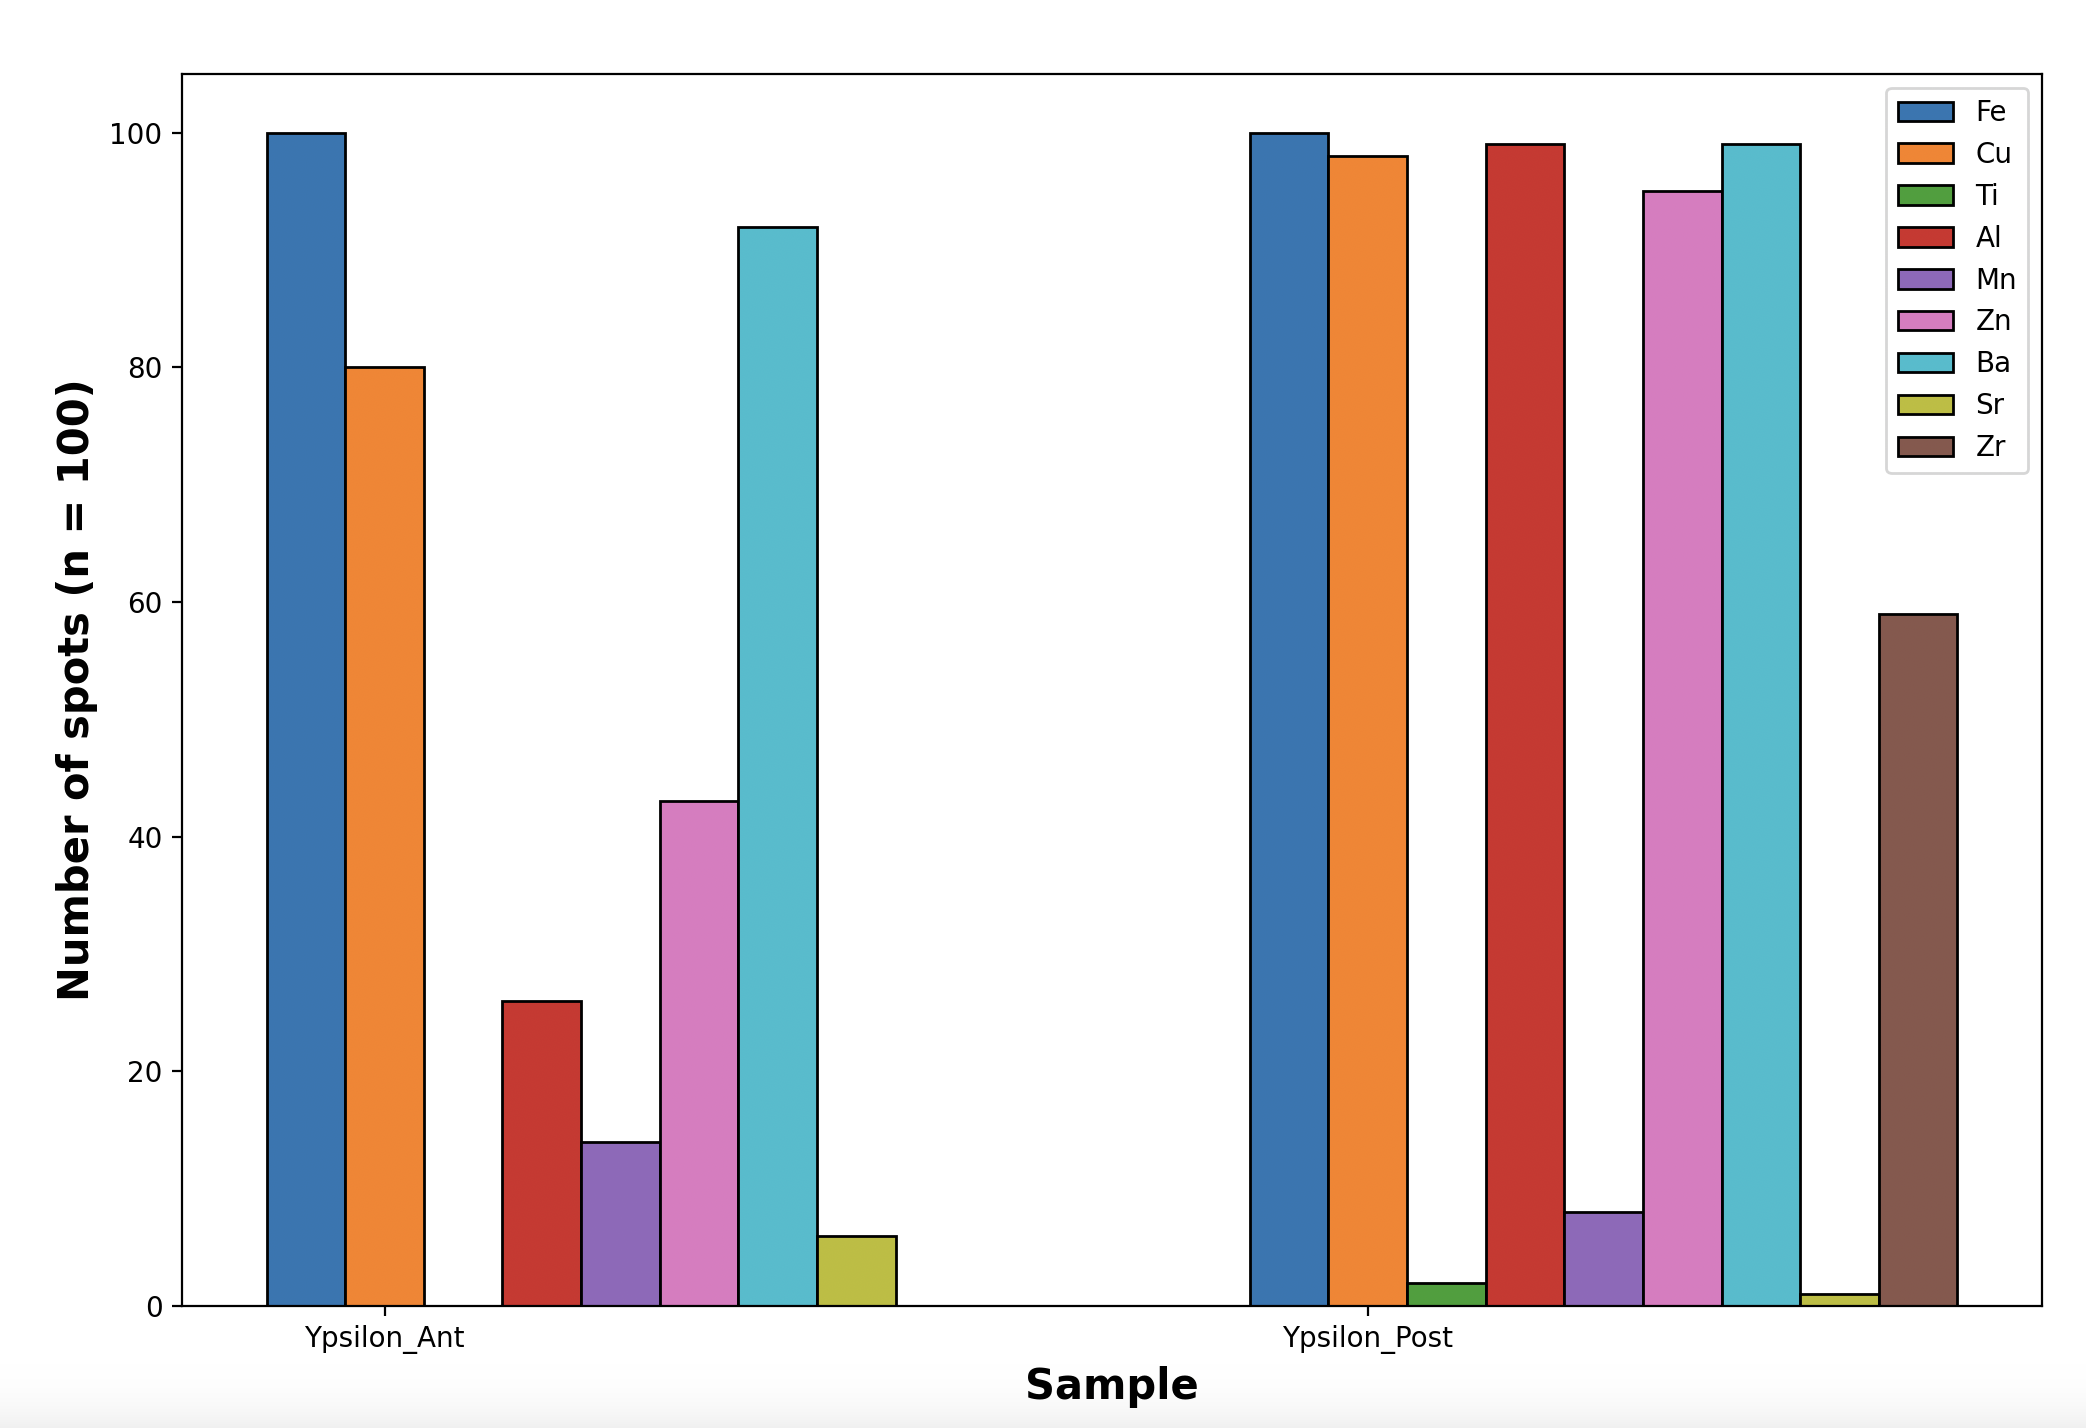
\includegraphics[scale=0.27]{images/Ypsilon_HM.png}
    \caption{Grouped bar chart of Ypsilon sample.}
    \label{fig:Ypsilon_HM}
\end{figure} 

\begin{figure}[H]
\centering
    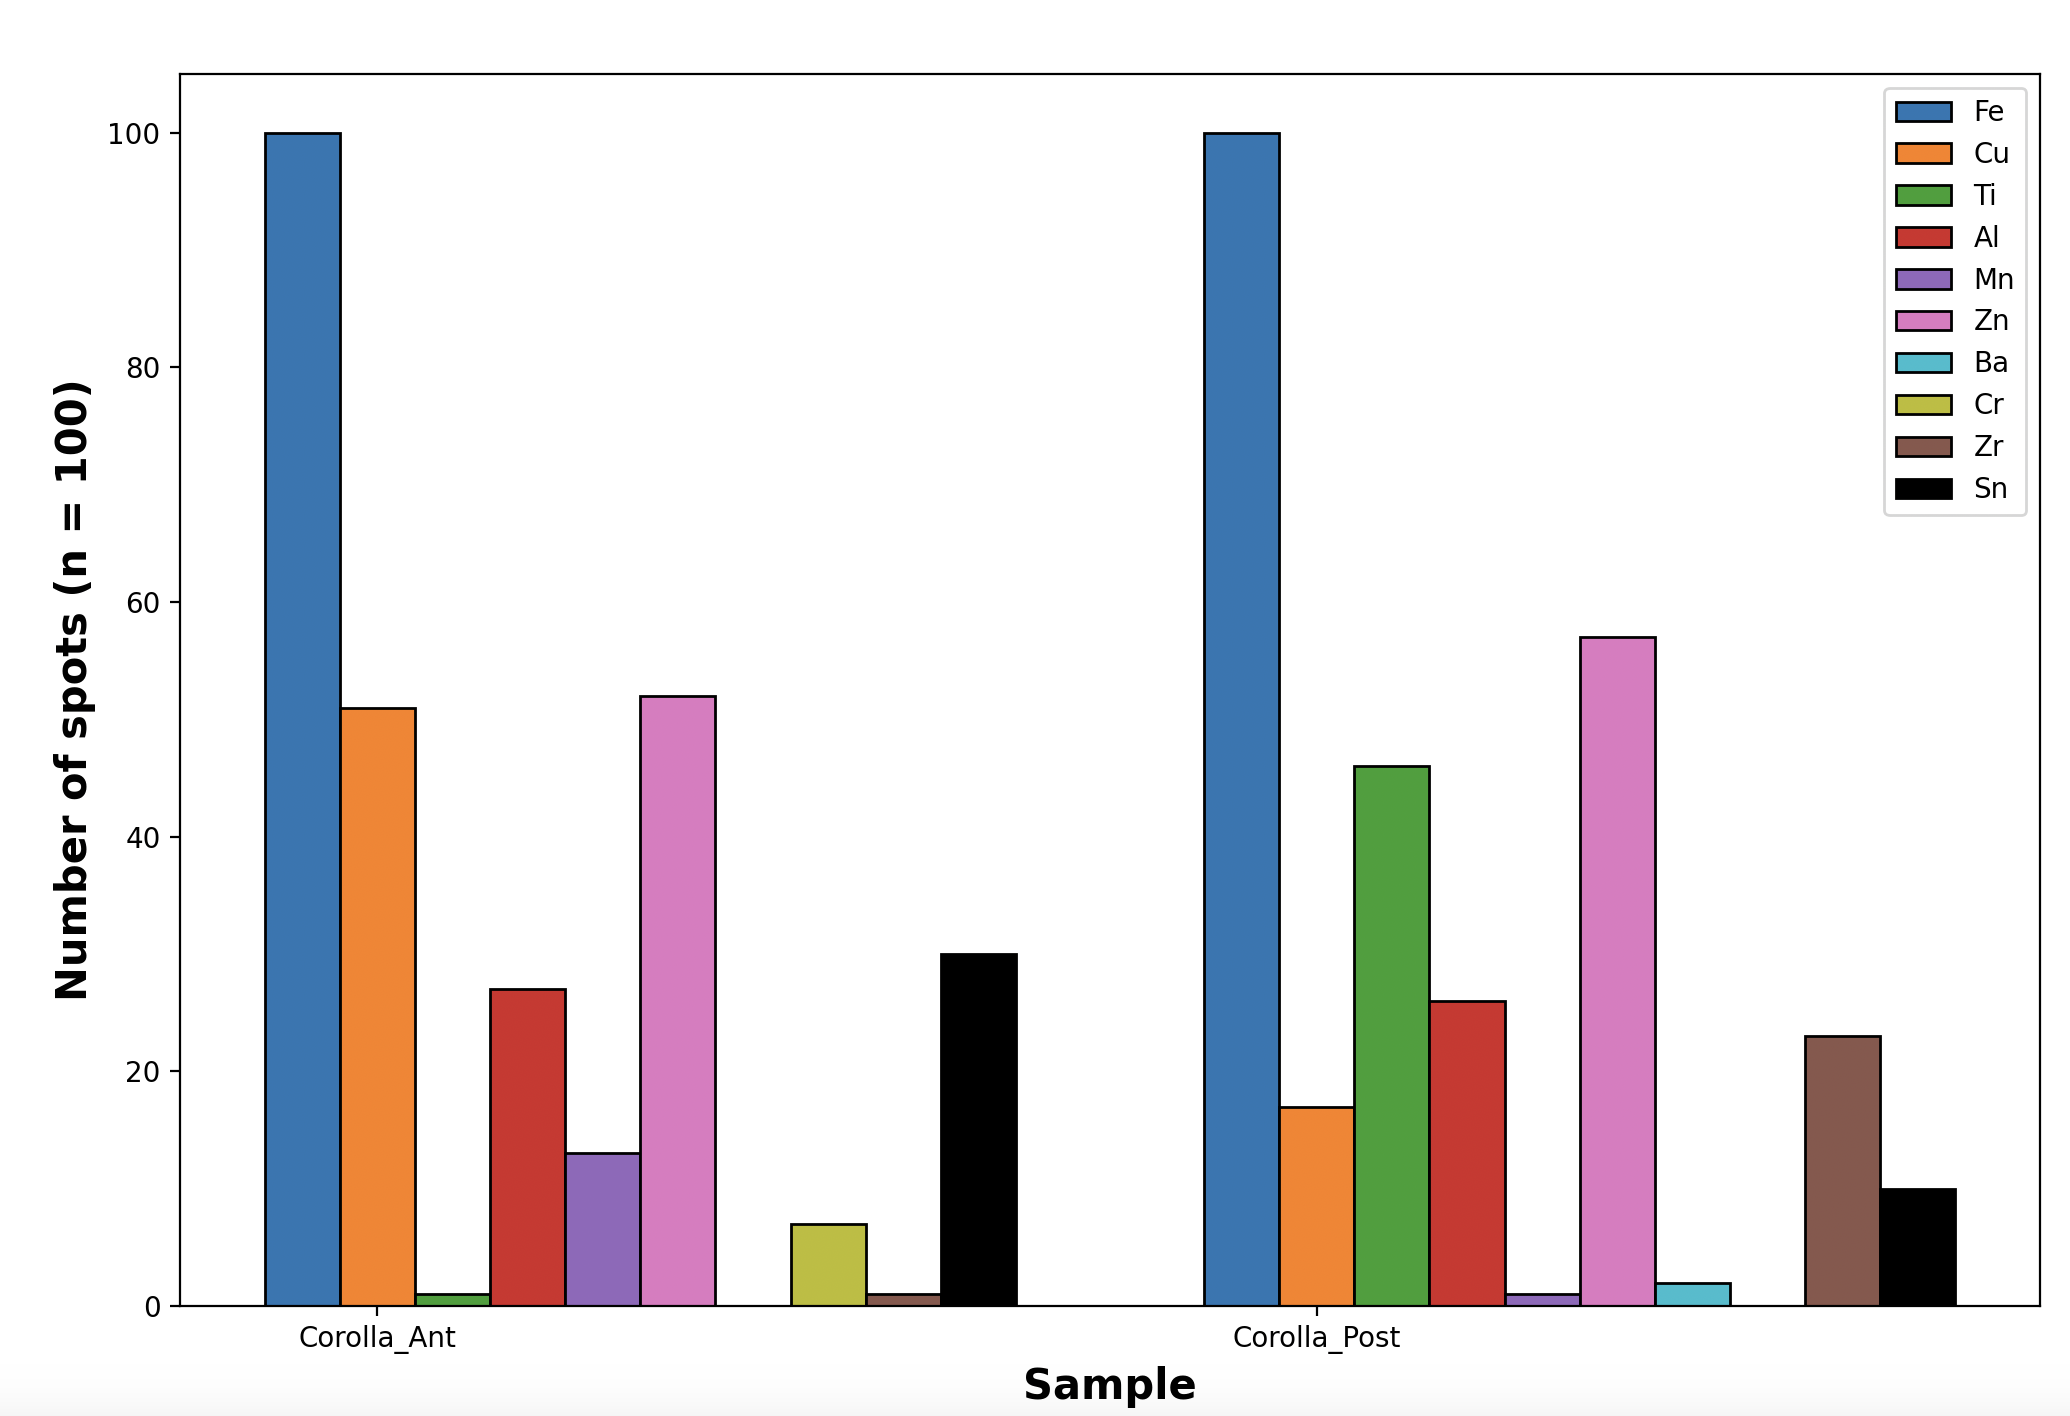
\includegraphics[scale=0.27]{images/Corolla_HM.png}
    \caption{Grouped bar chart of Corolla sample.}
    \label{fig:Corolla_HM}
\end{figure} 

\subsection{Chemical Analysis}

The chemical analysis was performed on a total of 10 sites per sample. Each site revealed a variety of elements, with some present in higher quantities than others. \\
To summarize the chemical composition of the samples, only the elements present in higher quantities and at more sites were considered. For each element, the mean of the different measurements was calculated, followed by the standard deviation ($\sigma (n-1)$) to assess the variation in the quantity of the element from the mean.\\
In each table, powders from the anterior (Ant) and posterior (Post) brakes of the same car were displayed together. If a specific element was detected in only one of the two samples, the symbol '-' was used to indicate its absence in the other one.

\begin{table}[H]\centering
  \begin{tabular}{lcccc}
    \toprule
    \multirow{2}{*}[-0.5\dimexpr \aboverulesep + \belowrulesep + \cmidrulewidth]{Panda}
    & \multicolumn{2}{c}{Ant} & \multicolumn{2}{c}{Post} \\
    \cmidrule(l){2-3} \cmidrule(l){4-5}
    & Mean (wt\%) & $\sigma (n-1)$ & Mean (wt\%) & $\sigma (n-1)$ \\
    \midrule
    O & 30.64 & 3.81 & 41.67 & 13.07 \\
    Na & 3.77 & 4.22 & 1.76 & 3.50 \\
    Mg & 0.43 & 0.75 & - & - \\
    Al & 1.32 & 4.06 & 1.81 & 1.40 \\
    Si & 4.34 & 1.34 & 3.66 & 1.60 \\
    P & 0.90 & 0.28 & 0.38 & 0.42 \\
    S & 5.01 & 3.78 & 3.74 & 4.60 \\
    Ca & 0.83 & 0.65 & 2.94 & 1.66 \\
    Mn & 0.30 & 0.32 & 0.06 & 0.16 \\
    Fe & 49.15 & 12.09 & 38.90 & 14.02 \\
    Cu & 0.91 & 0.44 & 1.25 & 2.21 \\
    Zn & - & - & 1.02 & 0.49 \\
    Ba & 2.84 & 4.87 & 2.13 & 1.16 \\
    \bottomrule
  \end{tabular}
    \caption{Main elements detected into the samples Panda Ant and Post, with mean and $\sigma (n-1)$.}
    \label{fig:Elements_Panda}
\end{table}

\begin{table}[H]\centering
  \begin{tabular}{lcccc}
    \toprule
    \multirow{2}{*}[-0.5\dimexpr \aboverulesep + \belowrulesep + \cmidrulewidth]{500X}
    & \multicolumn{2}{c}{Ant} & \multicolumn{2}{c}{Post} \\
    \cmidrule(l){2-3} \cmidrule(l){4-5}
    & Mean (wt\%) & $\sigma (n-1)$ & Mean (wt\%) & $\sigma (n-1)$ \\
    \midrule
    O & 45.17 & 11.66 & 48.88 & 9.15 \\
    Na & 0.76 & 2.07 & 0.67 & 1.41 \\
    Mg & 0.47 & 0.84 & - & - \\
    Al & 0.73 & 1.00 & 0.87 & 0.62 \\
    Si & 3.44 & 5.85 & 3.52 & 1.57 \\
    P & 0.22 & 0.37 & - & - \\
    S & 3.30 & 4.78 & 3.97 & 1.43 \\
    Cl & - & - & 0.42 & 0.35 \\
    Ca & 0.37 & 0.21 & 1.10 & 1.71 \\
    Fe & 41.07 & 13.04 & 19.45 & 12.00 \\
    Cu & 2.48 & 0.99 & 6.86 & 7.46 \\
    Zn & 0.90 & 0.55 & 2.19 & 0.77 \\
    Zr & 0.20 & 1.11 & 1.62 & 2.64 \\
    Sn & 0.29 & 0.37 & 2.42 & 1.82 \\
    Ba & - & - & 6.50 & 2.98 \\
    \bottomrule
  \end{tabular}
    \caption{Main elements detected into the samples 500X Ant and Post, with mean and $\sigma (n-1)$.}
    \label{fig:Elements_500X}
\end{table}

\begin{table}[H]\centering
  \begin{tabular}{lcccc}
    \toprule
    \multirow{2}{*}[-0.5\dimexpr \aboverulesep + \belowrulesep + \cmidrulewidth]{500L}
    & \multicolumn{2}{c}{Ant} & \multicolumn{2}{c}{Post} \\
    \cmidrule(l){2-3} \cmidrule(l){4-5}
    & Mean (wt\%) & $\sigma (n-1)$ & Mean (wt\%) & $\sigma (n-1)$ \\
    \midrule
    O & 41.90 & 11.19 & 30.82 & 3.31 \\
    Na & 1.12 & 3.65 & 2.34 & 4.03 \\
    Al & 0.38 & 2.00 & 1.75 & 1.32 \\
    Si & 3.02 & 3.88 & 4.10 & 2.54 \\
    P & 0.32 & 0.35 & - & - \\
    S & 2.75 & 2.86 & 5.40 & 2.81 \\
    Cl & 0.29 & 0.35 & - & - \\
    Cr & 0.05 & 0.09 & - & - \\
    Ca & - & - & 2.53 & 0.70 \\
    Mn & 0.30 & 0.20 & - & - \\
    Fe & 42.25 & 13.85 & 47.56 & 8.14 \\
    Cu & 3.33 & 1.20 & 1.17 & 0.40 \\
    Zn & 2.43 & 3.93 & 0.82 & 0.52 \\
    Zr & 0.76 & 3.81 & - & - \\
    Sn & 0.88 & 1.21 & - & - \\
    Ba & - & - & 3.13 & 1.42 \\
    \bottomrule
  \end{tabular}
    \caption{Main elements detected into the samples 500L Ant and Post, with mean and $\sigma (n-1)$.}
    \label{fig:Elements_500L}
\end{table}

\begin{table}[H]\centering
  \begin{tabular}{lcccc}
    \toprule
    \multirow{2}{*}[-0.5\dimexpr \aboverulesep + \belowrulesep + \cmidrulewidth]{Ypsilon}
    & \multicolumn{2}{c}{Ant} & \multicolumn{2}{c}{Post} \\
    \cmidrule(l){2-3} \cmidrule(l){4-5}
    & Mean (wt\%) & $\sigma (n-1)$ & Mean (wt\%) & $\sigma (n-1)$ \\
    \midrule
    O & 29.29 & 2.30 & 33.47 & 4.08 \\
    Na & 1.73 & 2.92 & 1.21 & 2.39 \\
    Mg & 1.56 & 1.63 & 1.09 & 2.28 \\
    Al & 0.31 & 0.76 & 4.50 & 3.32 \\
    Si & 3.82 & 0.95 & 7.59 & 6.22 \\
    P & 0.14 & 0.28 & 0.98 & 1.85 \\
    S & 4.27 & 2.34 & 3.31 & 2.08 \\
    Cl & 0.08 & 0.23 & 0.77 & 0.60 \\
    K & - & - & 1.39 & 2.80 \\
    Ca & 0.80 & 3.31 & 5.40 & 5.08 \\
    Mn & 0.07 & 0.17 & 0.04 & 0.23 \\
    Fe & 54.31 & 9.84 & 28.80 & 10.37 \\
    Cu & 0.56 & 0.52 & 1.45 & 0.50 \\
    Zn & 0.35 & 0.55 & 2.12 & 1.07 \\
    Zr & - & - & 0.94 & 0.98 \\
    Ba & 2.25 & 3.93 & 5.86 & 2.33 \\
    \bottomrule
  \end{tabular}
    \caption{Main elements detected into the samples Ypsilon Ant and Post, with mean and $\sigma (n-1)$.}
    \label{fig:Elements_Ypsilon}
\end{table}

\begin{table}[H]\centering
  \begin{tabular}{lcccc}
    \toprule
    \multirow{2}{*}[-0.5\dimexpr \aboverulesep + \belowrulesep + \cmidrulewidth]{Corolla}
    & \multicolumn{2}{c}{Ant} & \multicolumn{2}{c}{Post} \\
    \cmidrule(l){2-3} \cmidrule(l){4-5}
    & Mean (wt\%) & $\sigma (n-1)$ & Mean (wt\%) & $\sigma (n-1)$ \\
    \midrule
    O & 29.72 & 3.60 & 34.69 & 6.13 \\
    Na & 1.82 & 3.58 & 0.80 & 2.32 \\
    Mg & 0.26 & 1.25 & 3.53 & 6.96 \\
    Al & 1.05 & 4.42 & 1.15 & 2.83 \\
    Si & 3.81 & 2.49 & 9.55 & 6.73 \\
    P & 0.52 & 0.72 & 0.48 & 2.01 \\
    S & 4.03 & 3.10 & 3.43 & 2.95 \\
    Cl & - & - & 0.67 & 3.09 \\
    K & - & - & 1.12 & 4.25 \\
    Ca & 0.24 & 0.34 & 4.09 & 10.18 \\
    Cr & 0.39 & 17.98 & - & - \\
    Ti & - & - & 2.82 & 4.15 \\
    Fe & 55.90 & 11.74 & 34.03 & 21.15 \\
    Cu & 1.19 & 1.96 & 0.25 & 0.64 \\
    Zn & 0.62 & 0.77 & 1.33 & 2.77 \\
    Zr & - & - & 1.44 & 4.95 \\
    Sn & 0.32 & 0.54 & 0.42 & 3.30 \\
    \bottomrule
  \end{tabular}
    \caption{Main elements detected into the samples Corolla Ant and Post, with mean and $\sigma (n-1)$.}
    \label{fig:Elements_Corolla}
\end{table}
\pagebreak

\subsection{Morphology}

All the samples exhibited a wide array of morphologies. Generally, the presence of agglomerates of particles of different sizes is very common. Given the diverse materials used in brake production, it is not surprising to find such a variety of morphologies. As previously mentioned, every component of brake pads plays a specific role in the braking system. \\
Figure \ref{fig:Layers} shows the typical composition of brake pads, highlighting that larger particles act as abrasives while smaller particles function as fillers. Elongated morphology is also common due to the presence of reinforcement fibers.

\begin{figure}[H]
\centering
    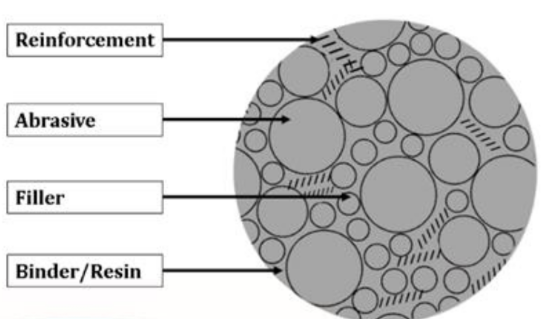
\includegraphics[scale=0.85]{images/layers.png}
    \caption{Different components present in brakes \cite{irawan2022overview}.}
    \label{fig:Layers}
\end{figure}

In general, it was observed that the concentration of nanoparticles smaller than 100 nm in brake powders increases with the temperature of the cast iron disc. Submicron particles are formed by evaporation or condensation processes, followed by the subsequent aggregation of primary nanoparticles \cite{grigoratos2015brake}.\\
During SEM observations, most of the brake components were identified in all samples and classified according to their main morphology.\\

As evidenced by recent research on the characterization of vehicle brake emissions \cite{liati2019airborne}, coarse PM ranging from 10 µm to 2.5 µm predominantly appears as aggregates composed of particles of varying sizes and irregular shapes. \\
Single coarse particles were observed less frequently than fine particles, which range between 2.5 µm and 0.1 µm and sometimes occur separated from the aggregates.
In this study, aggregates were observed in both anterior and posterior brakes and in all of the sample regardless the type of car analyzed.

\begin{figure}[H]
\centering
\begin{subfigure}{.5\textwidth}
  \centering
  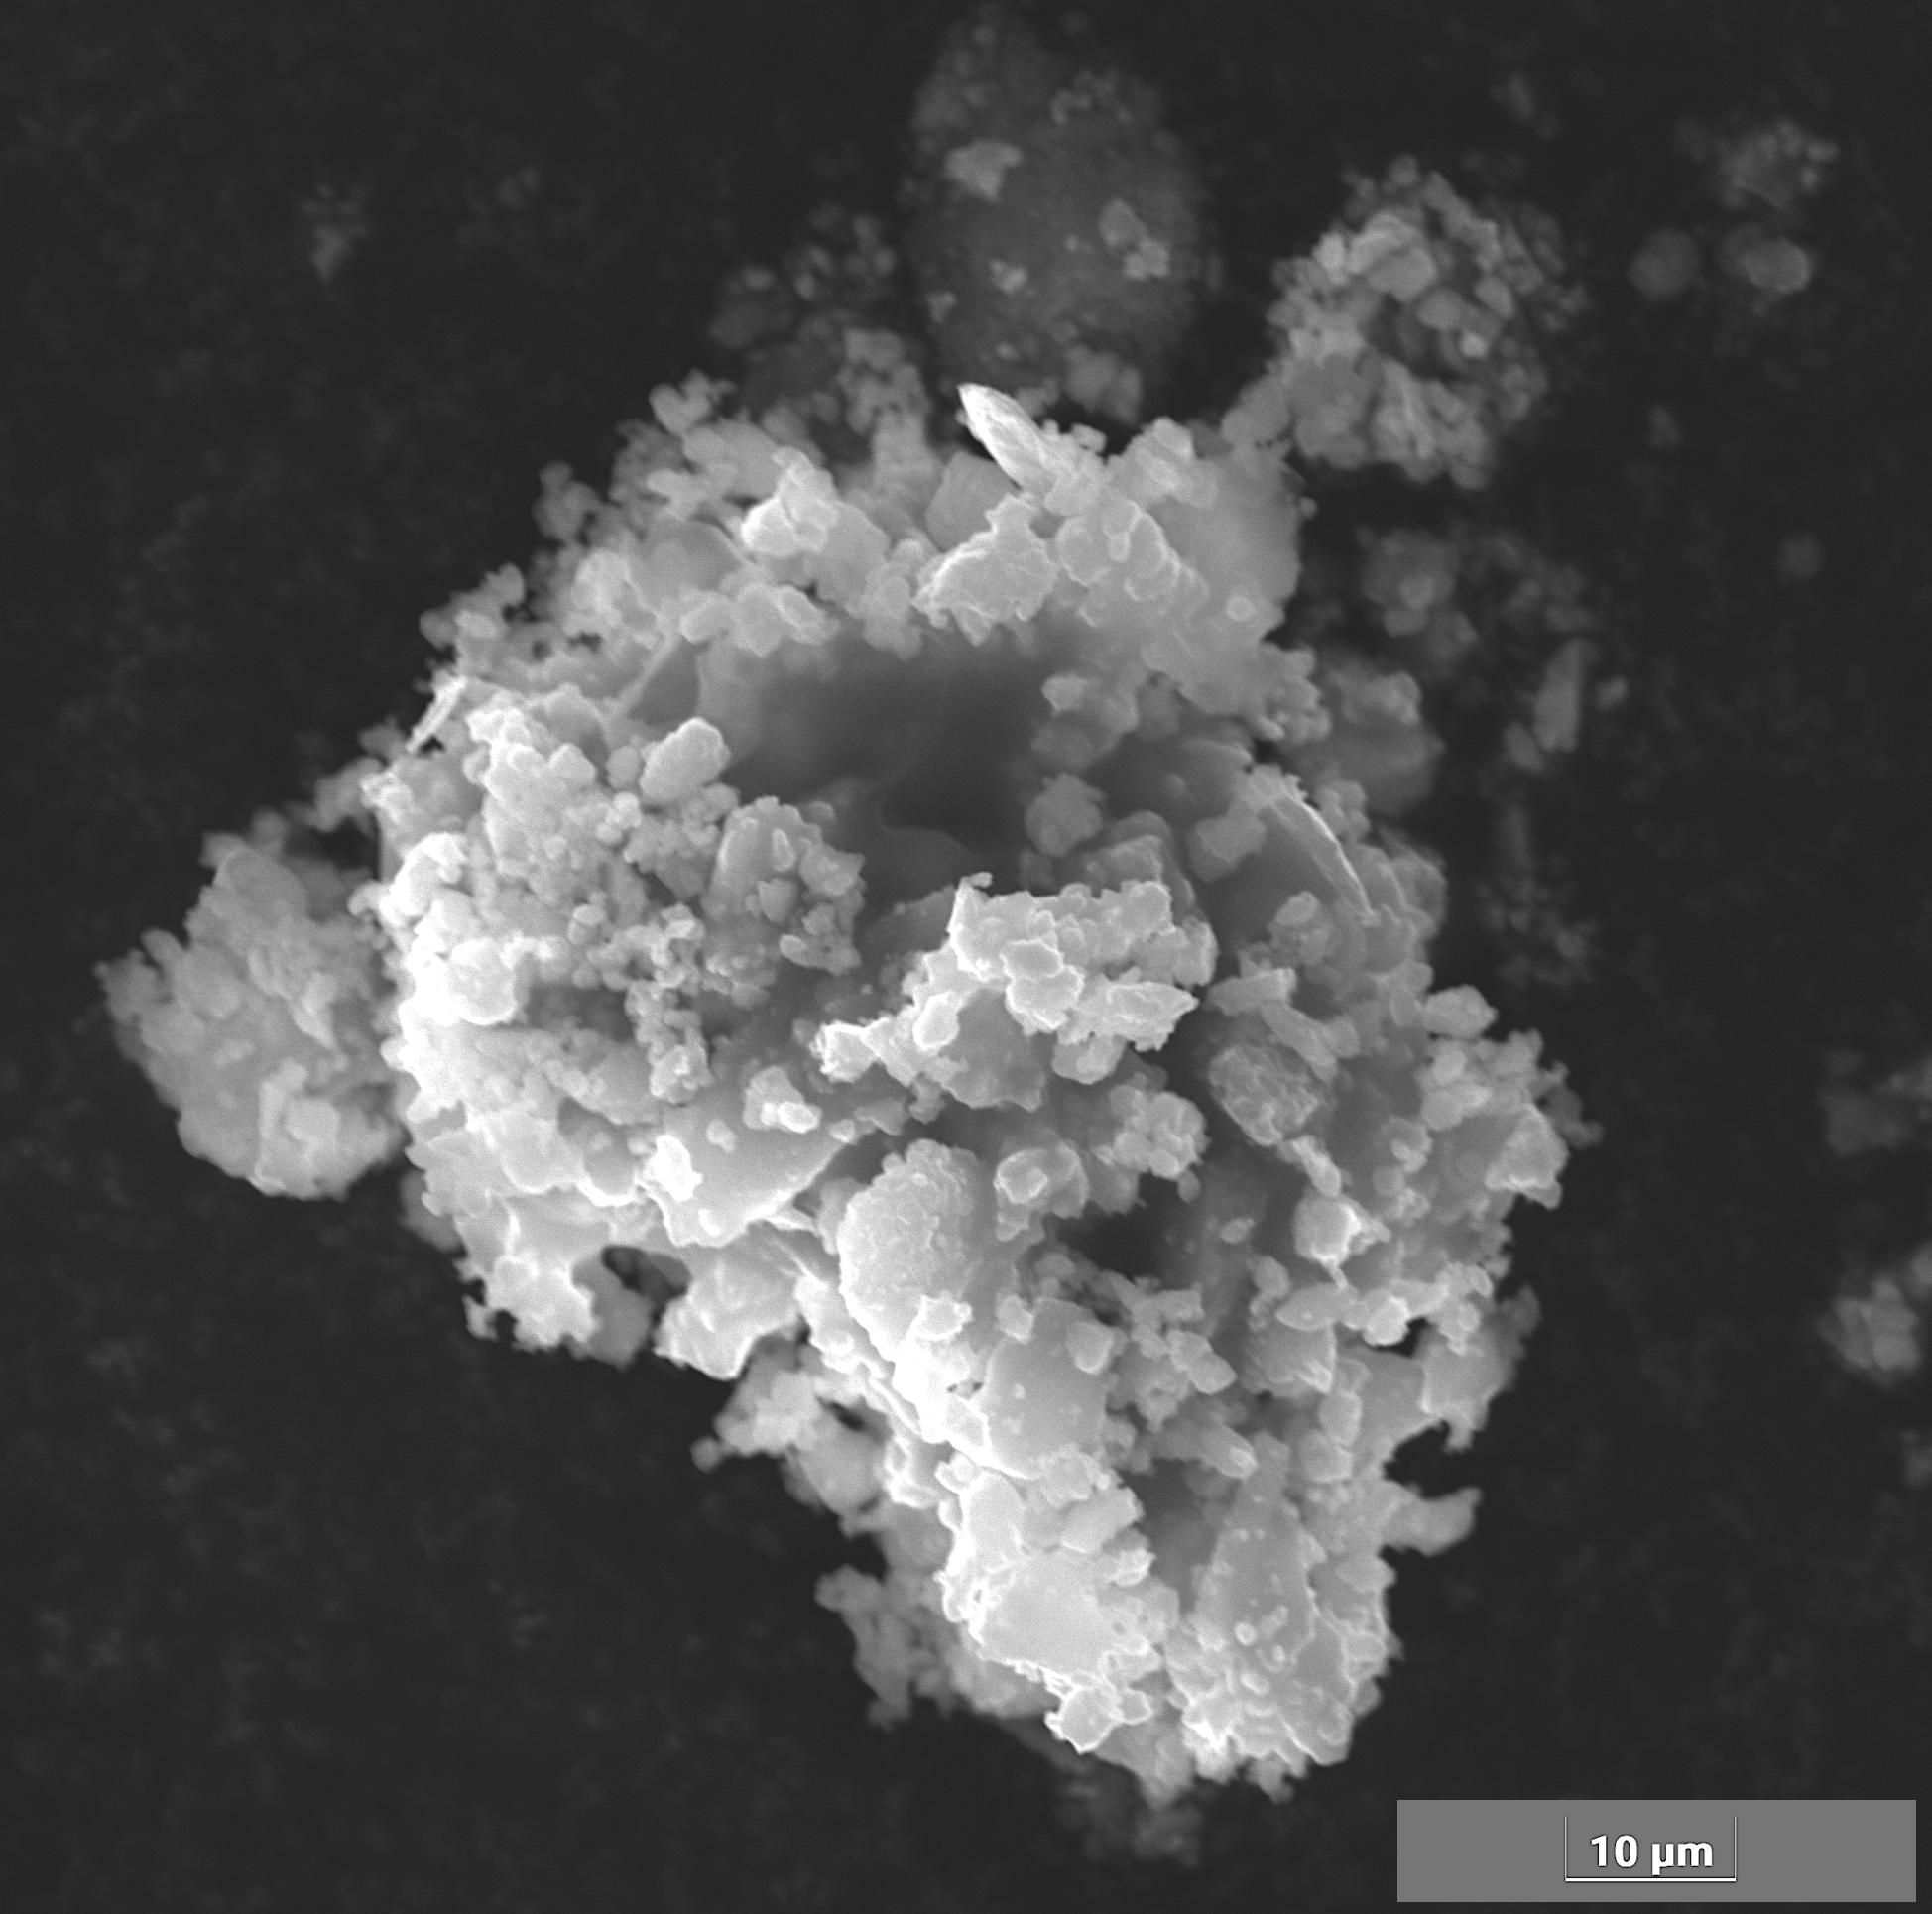
\includegraphics[width=1\linewidth]{images/500L-ANT05-copia.png}
  \caption{500L Ant}
  \label{fig:Aggregates_500L_Ant}
\end{subfigure}%
\begin{subfigure}{.5\textwidth}
  \centering
  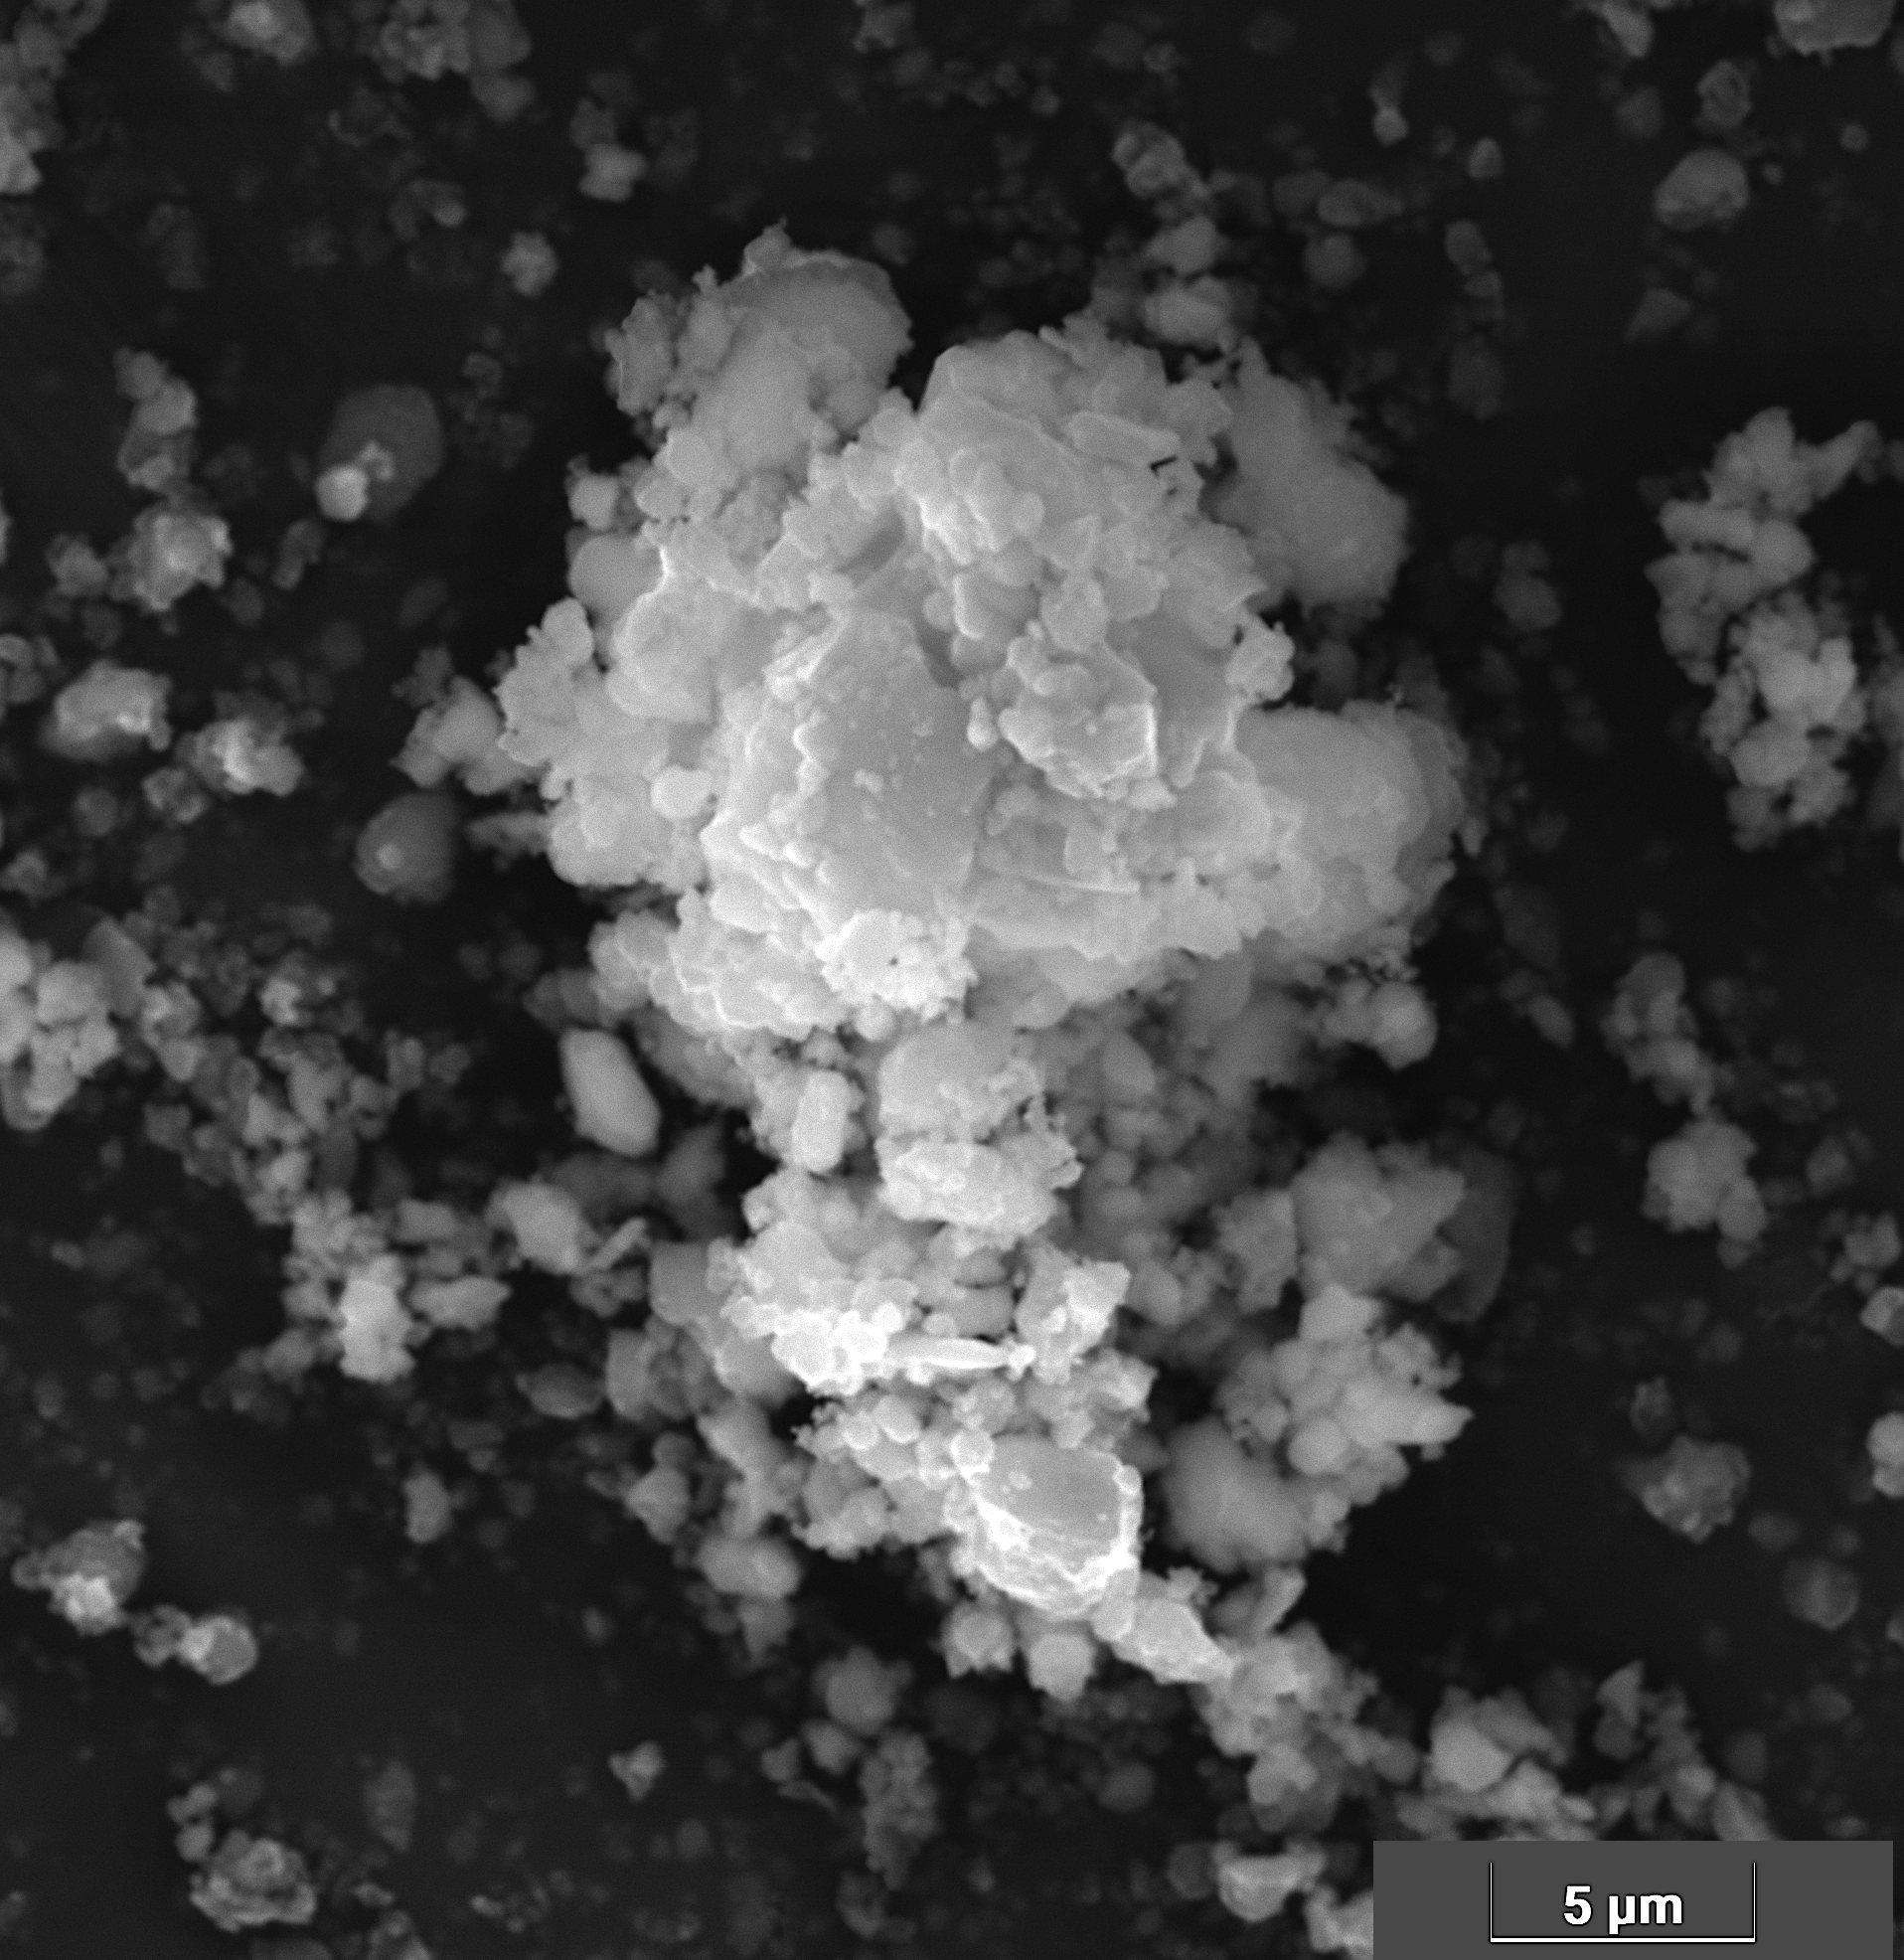
\includegraphics[width=0.97\linewidth]{images/YPSILON-ANT04.png}
  \caption{Ypsilon Ant}
  \label{fig:Aggregates_Y_Ant}
\end{subfigure}
\caption{Examples of aggregates found in the powders from anterior brakes of two different sample.}
\label{fig:Aggregates_Ant}
\end{figure}

\begin{figure}[H]
\centering
\begin{subfigure}{.5\textwidth}
  \centering
  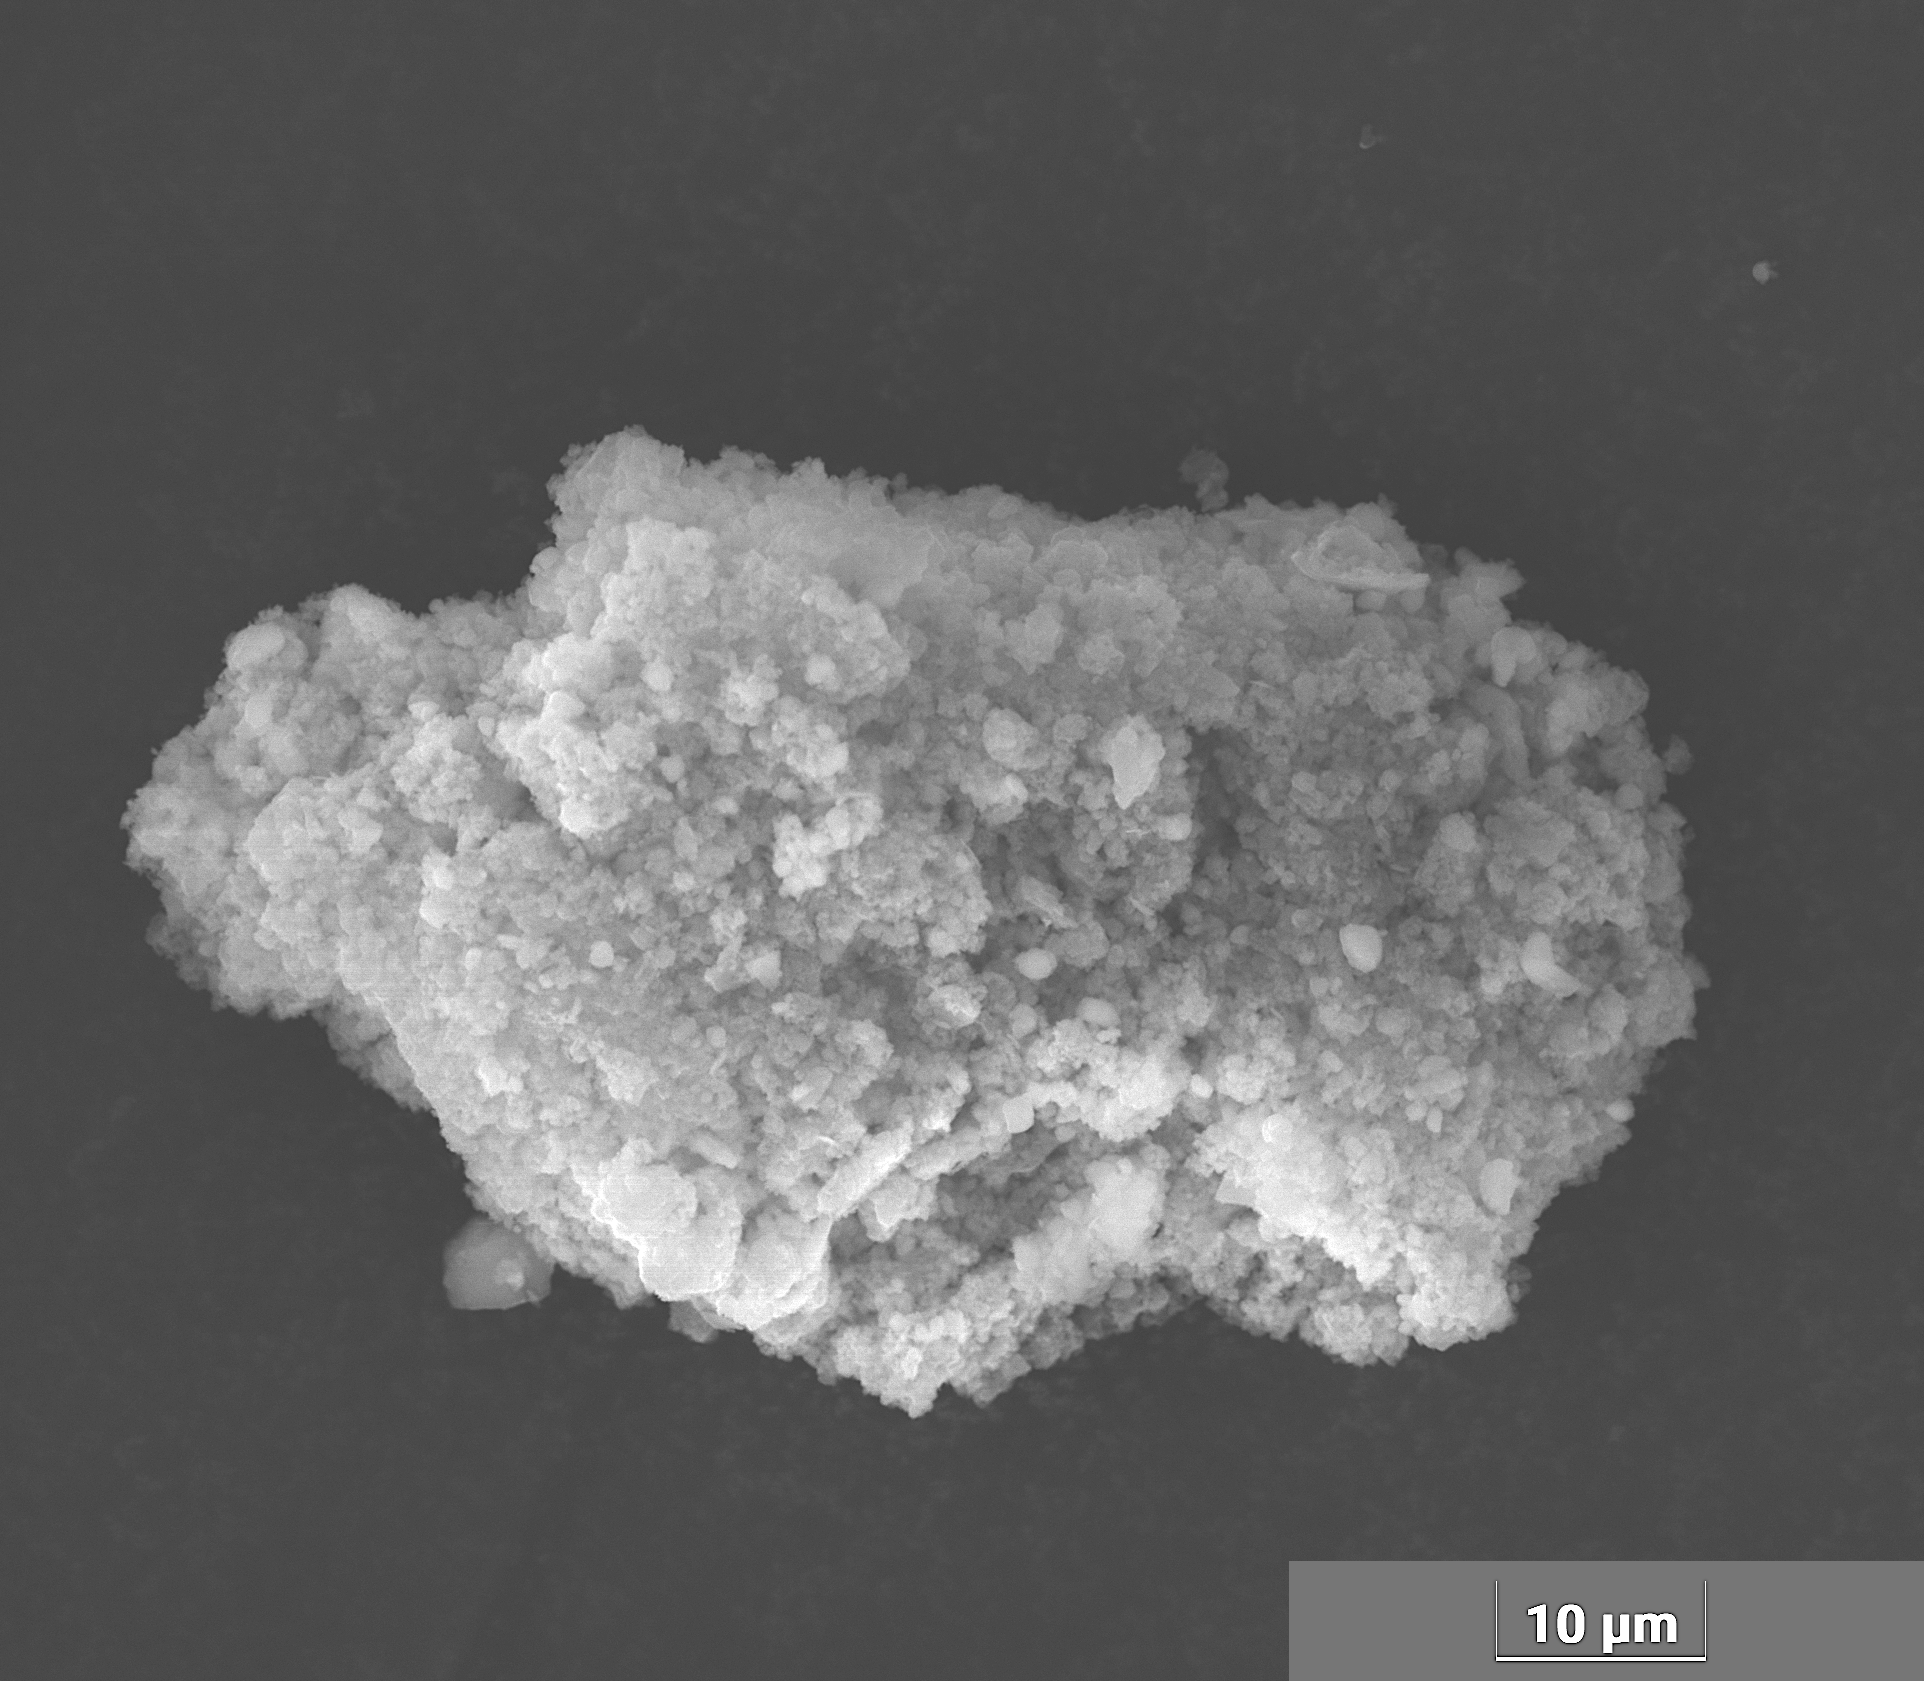
\includegraphics[width=1\linewidth]{images/COROLLA-POST01.png}
  \caption{Corolla Post}
  \label{fig:Aggregates_Corolla_Post}
\end{subfigure}%
\begin{subfigure}{.5\textwidth}
  \centering
  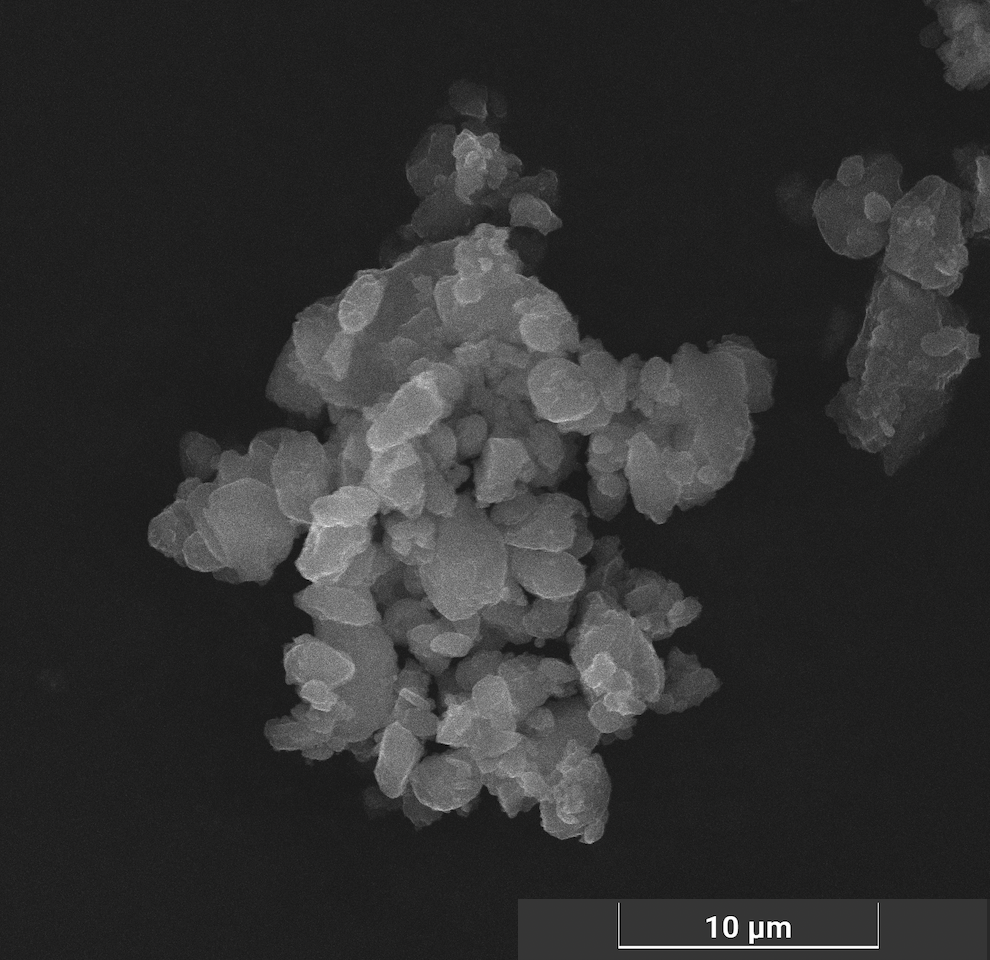
\includegraphics[width=0.9\linewidth]{images/PANDA-POST02.png}
  \caption{Panda Post}
  \label{fig:Aggregates_Panda_Post}
\end{subfigure}
\caption{Examples of aggregates found in the powders from posterior brakes of two different sample.}
\label{fig:Aggregates_Post}
\end{figure}

It is important to note that, the powders found on the surface of brakes, are synthetic material, as they are produced during braking rather than originating from natural sources. Therefore, to describe the various morphologies observed, the mechanisms by which wear debris is generated were used as a reference for this characterization .\\
In a related article such mechanisms are explained thoroughly, here an extract is reported as a reference:
\pagebreak
\blockquote[\cite{machinerylubricationAnatomyWear}]{
One of the most common ways platelet-shaped particles can occur is by normal and tangential forces through contacting asperities. \\

Wire or curl-shaped particles have been linked to cutting wear where one of the contacting surfaces possesses an asperity or lodged particle that is plastically rigid compared to the other surface from which the ribbon-shaped particle is gouged out.}

Based on this statement and another reference describing the shapes of various industrial particles \cite{ulusoy2023review}, the presence of different shapes among the samples, as shown below in Figures \ref{fig:Lamellar}, was identified.

\begin{figure}[H]
 \centering
    \begin{subfigure}{0.45\linewidth}
        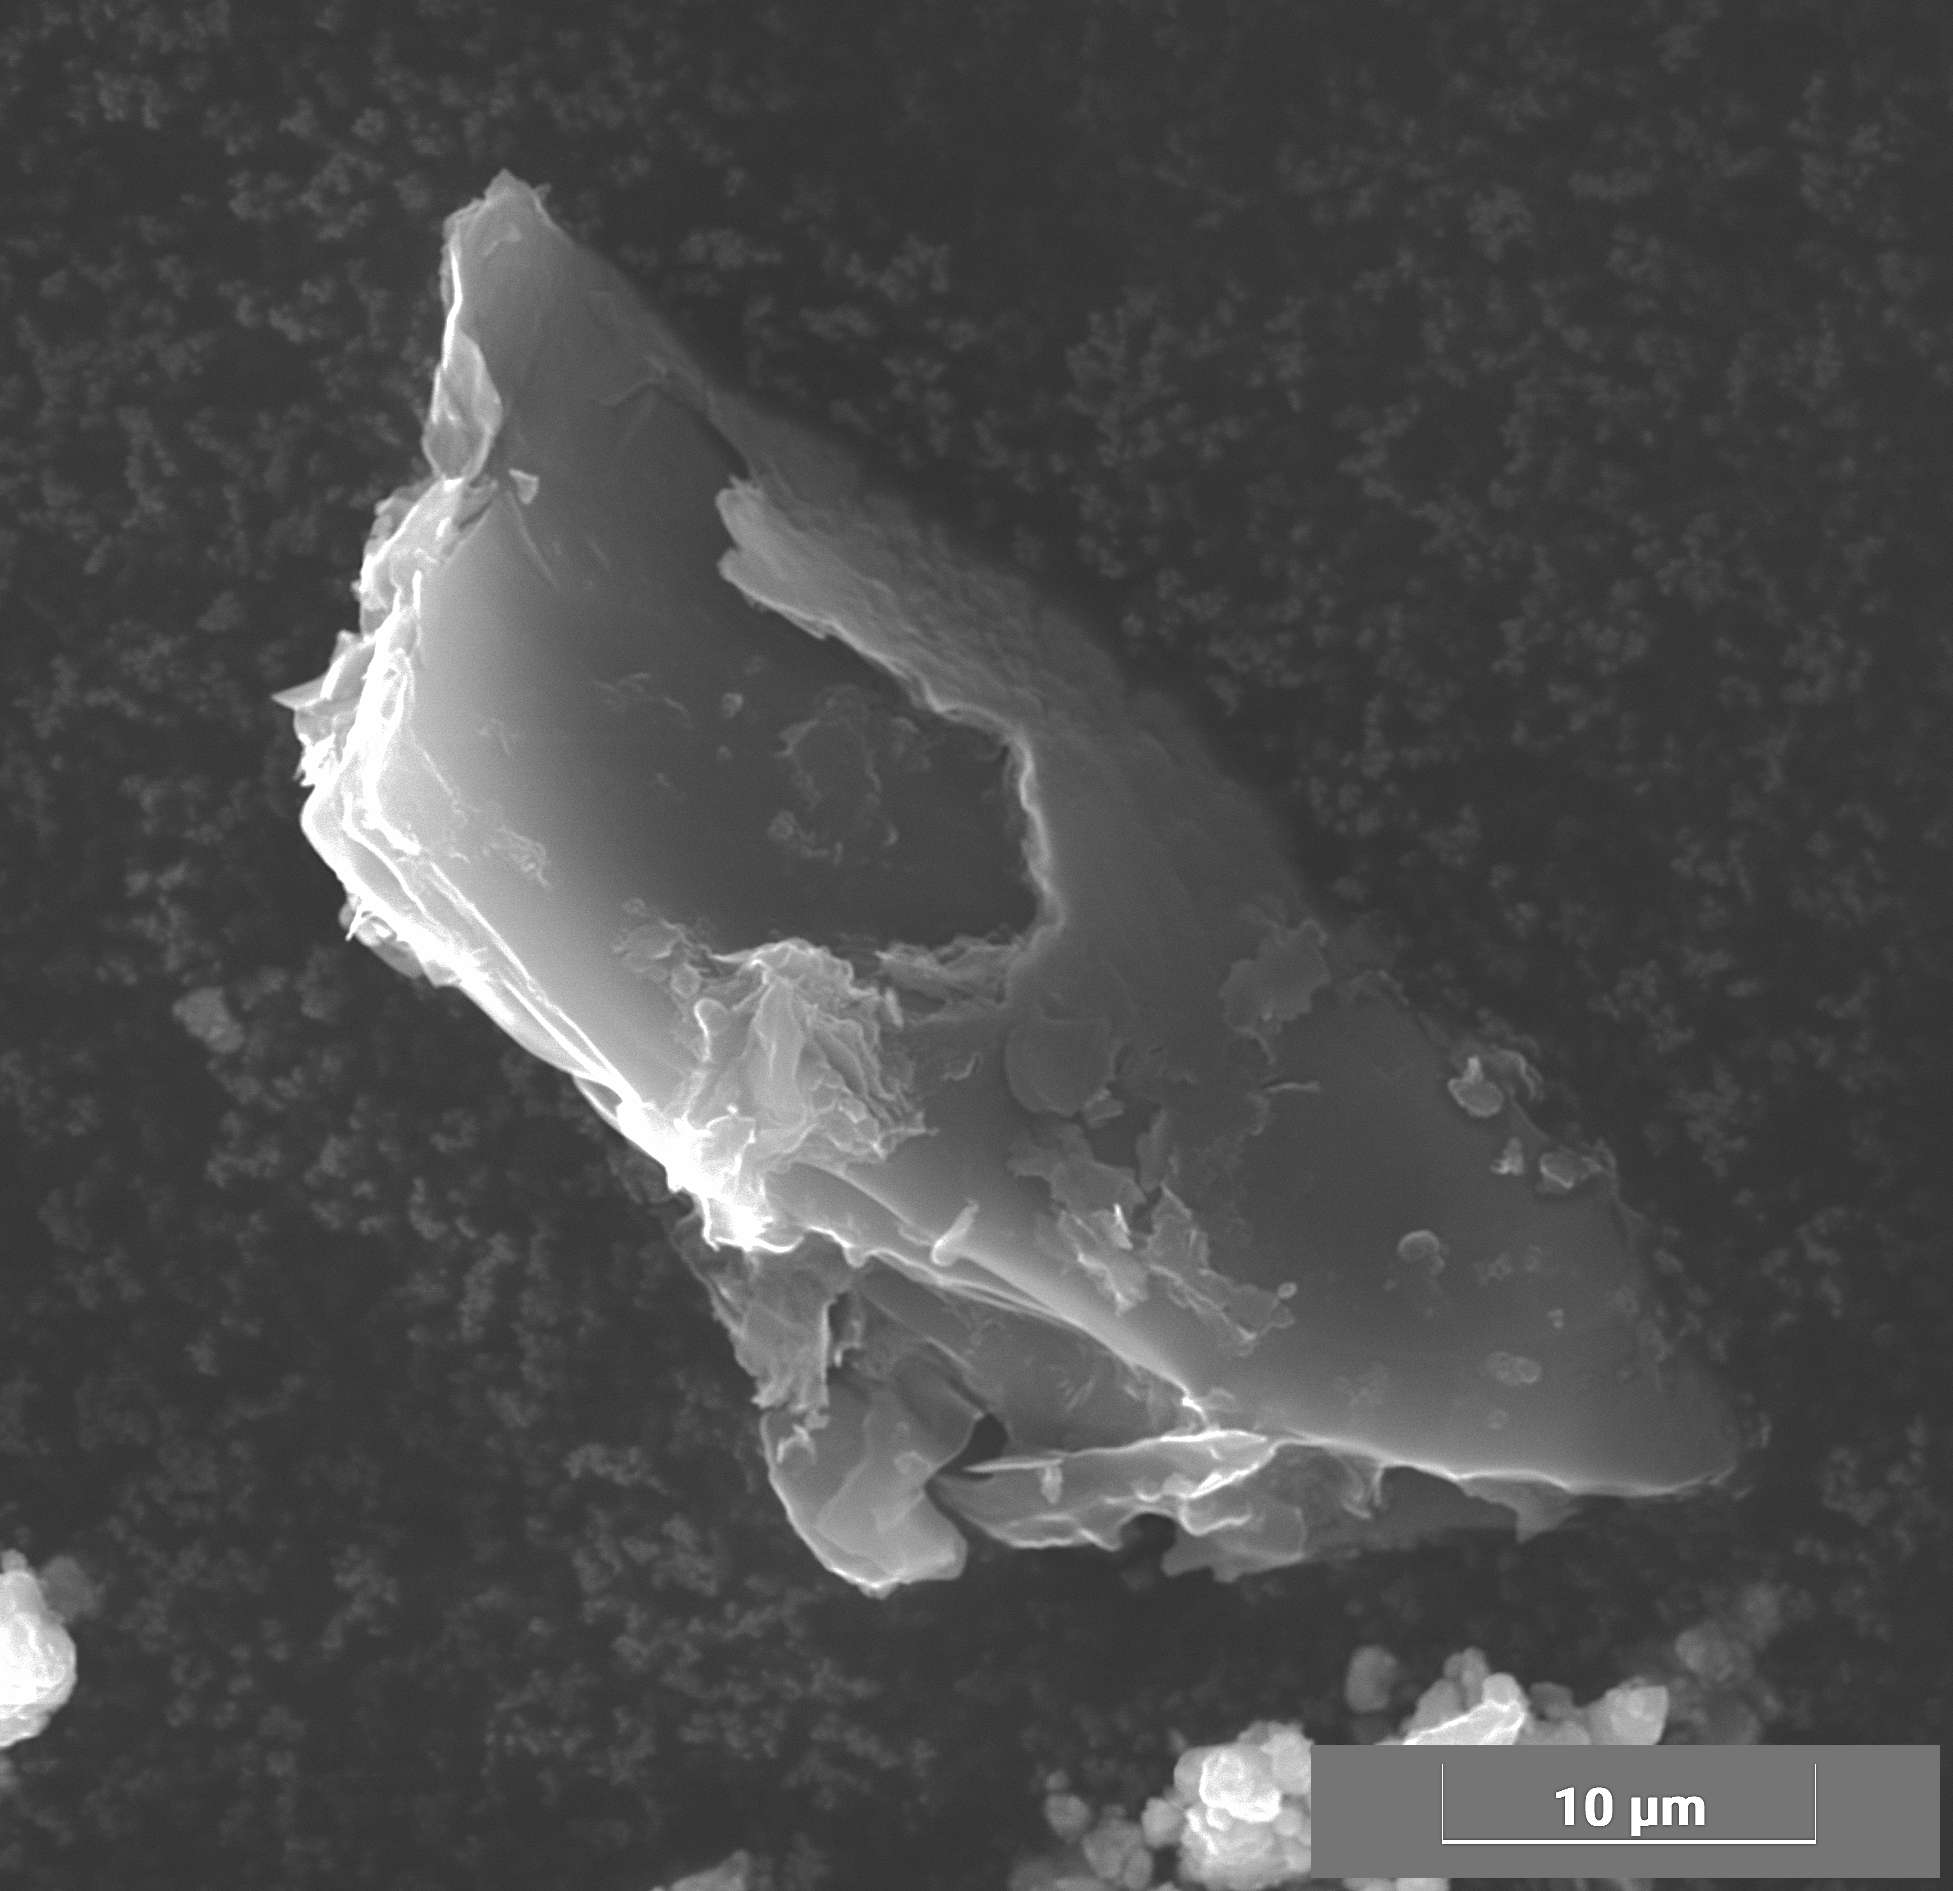
\includegraphics[width=\linewidth]{images/500L POST11 lamellar.png}
		\caption{500L Post}
		\label{fig:500L_Post_Lamellar}
	   \end{subfigure}
	   \begin{subfigure}{0.43\linewidth}
		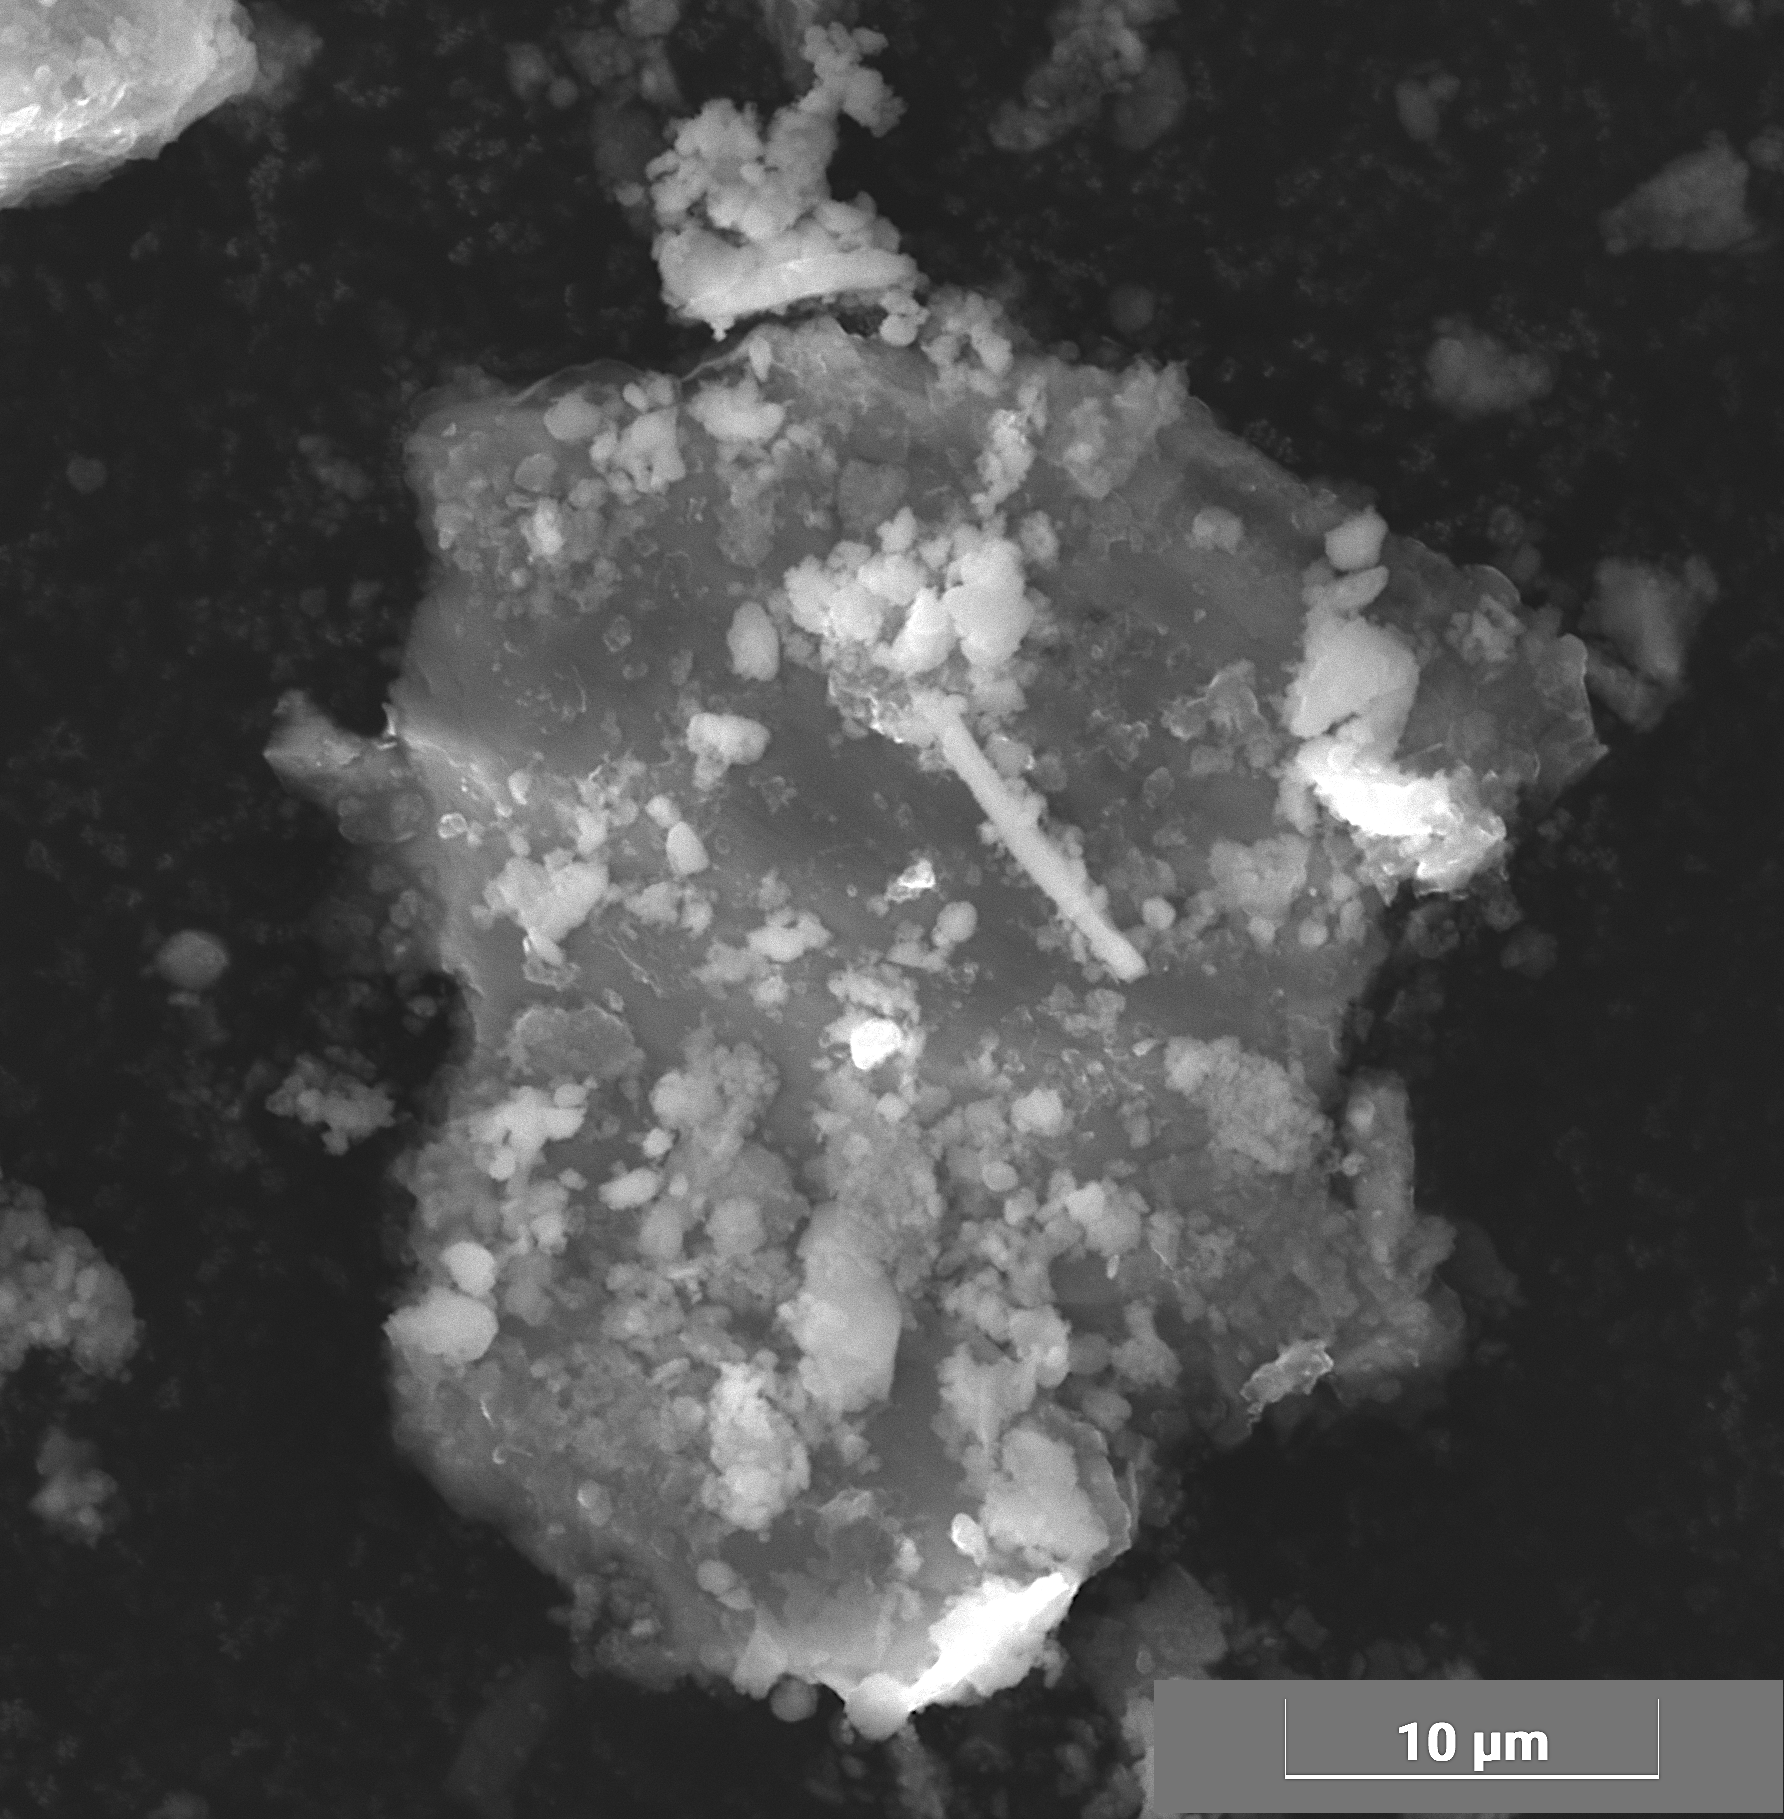
\includegraphics[width=\linewidth]{images/500X POST03 lamellar.png}
		\caption{500X Post}
		\label{fig:500X_Post_Lamellar}
	    \end{subfigure}
	\vfill
	     \begin{subfigure}{0.45\linewidth}
		 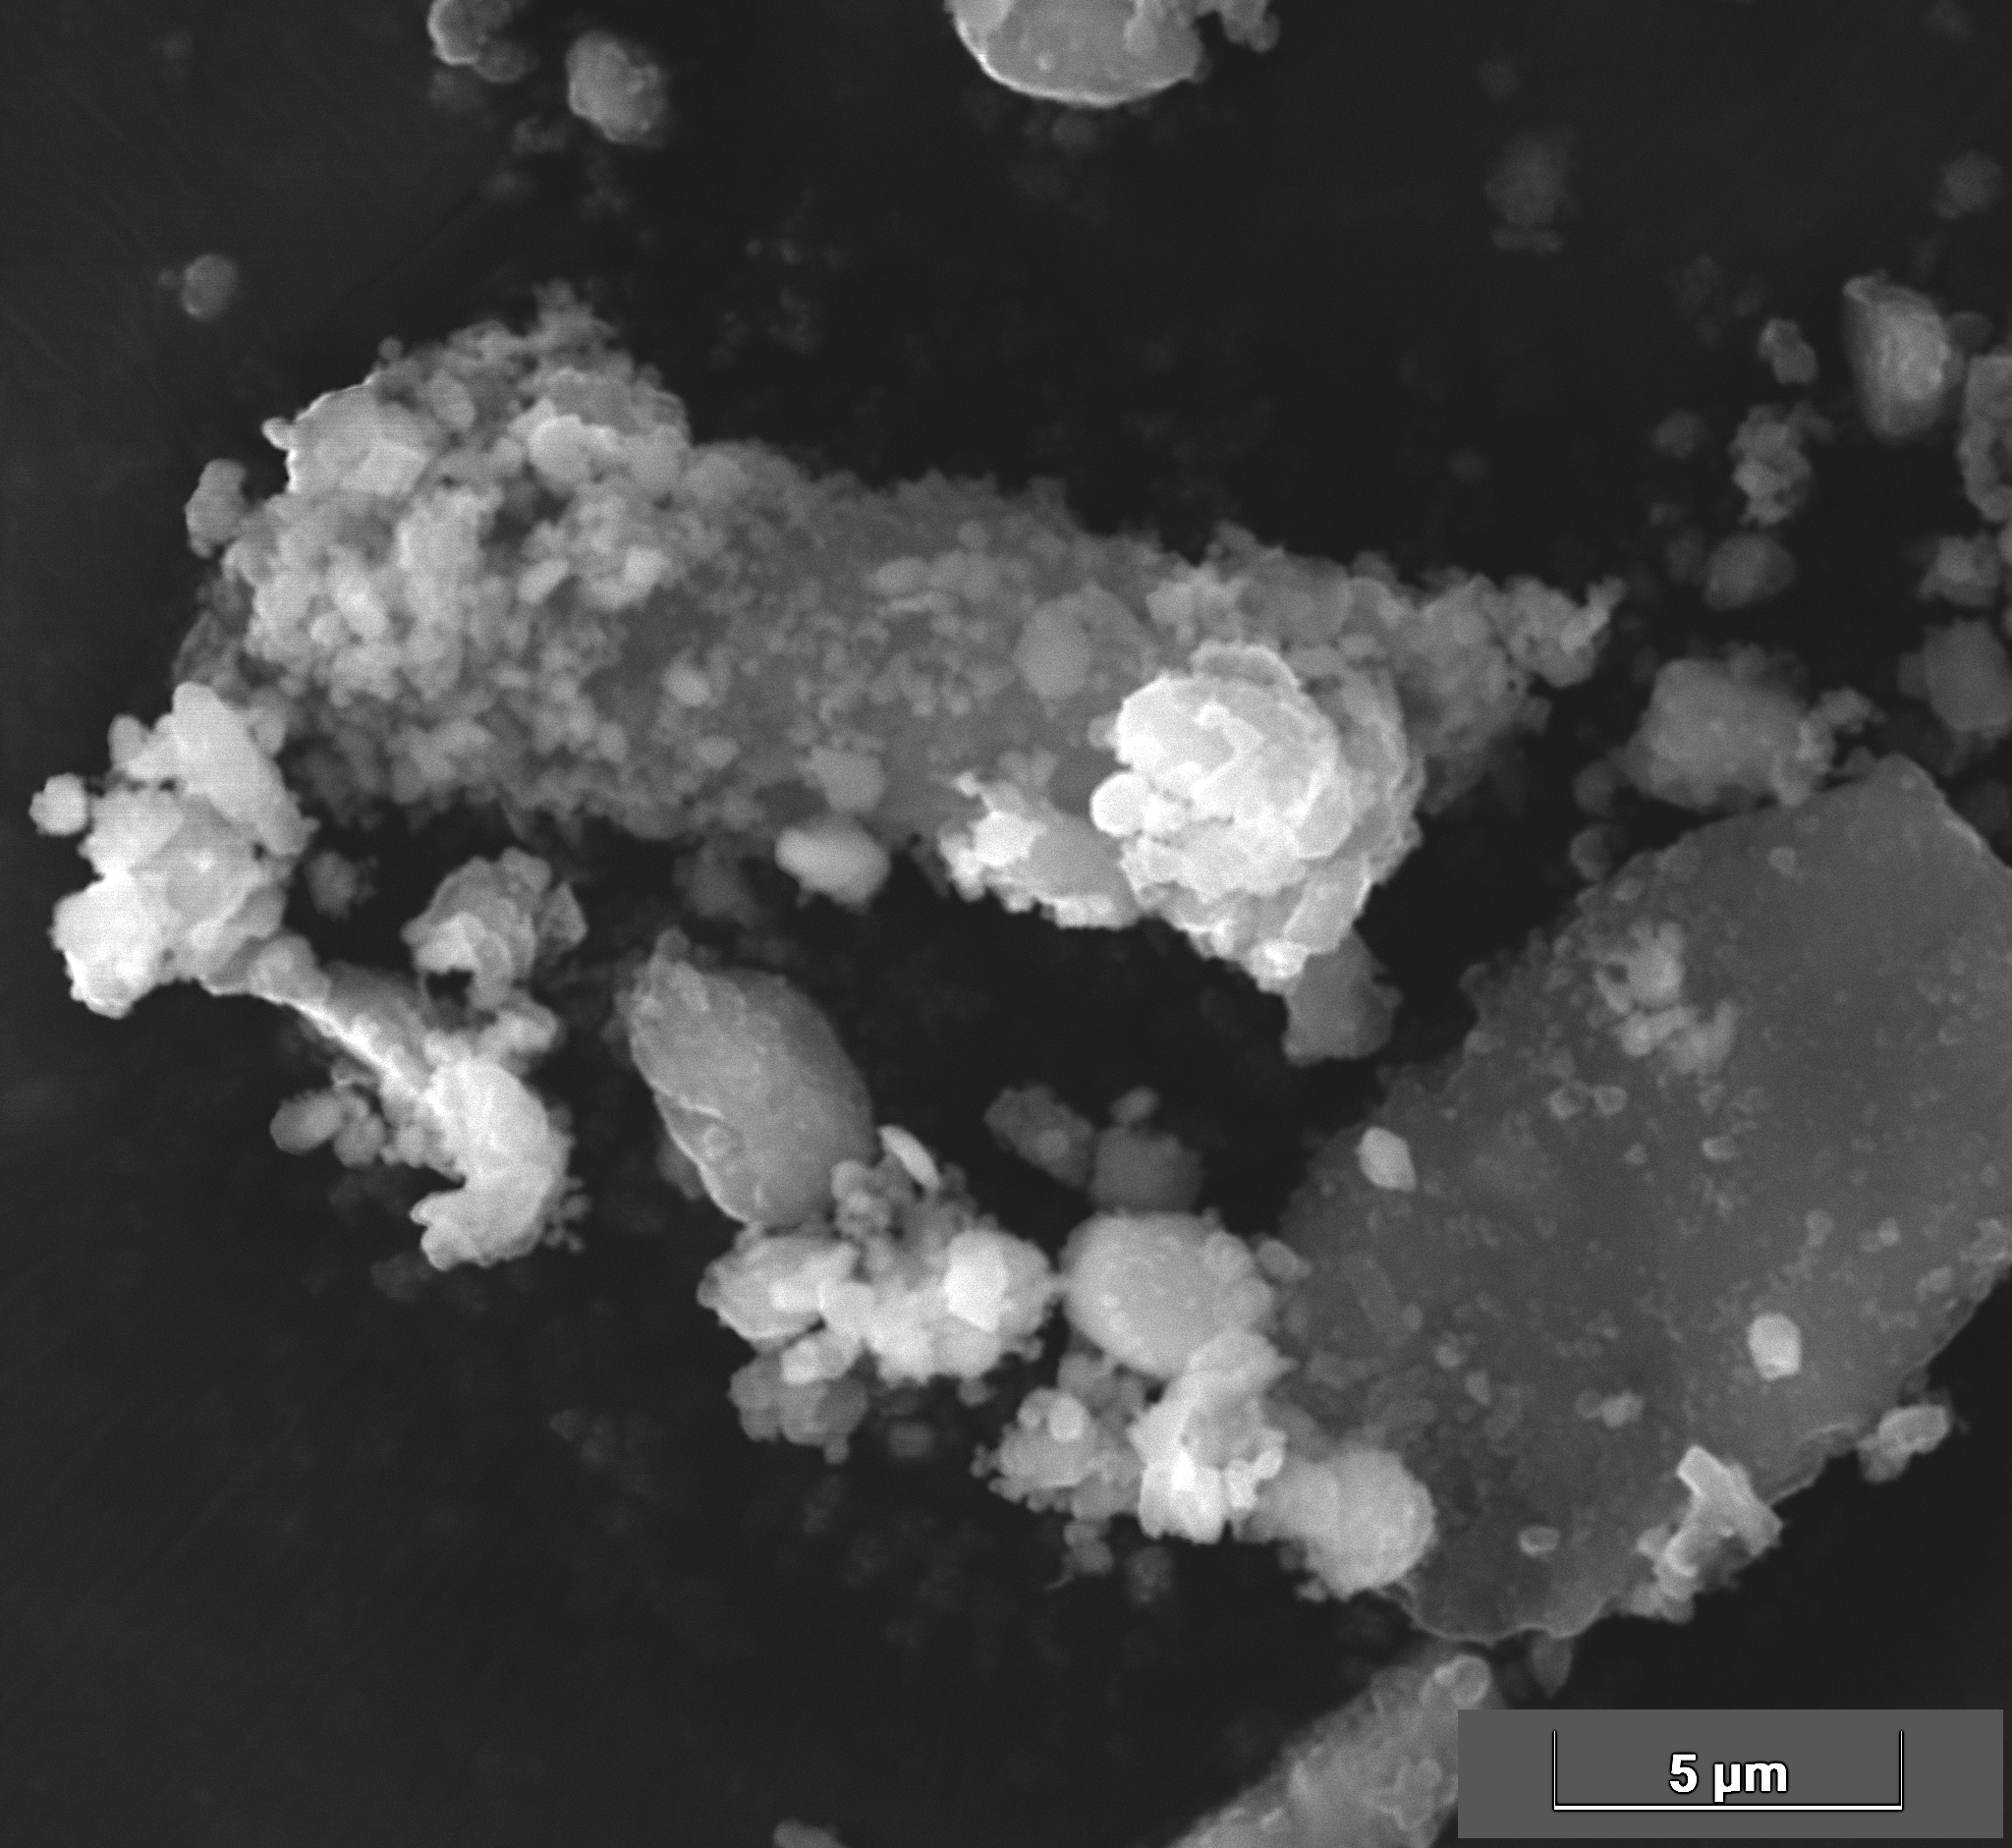
\includegraphics[width=\linewidth]{images/COROLLA ANT05 lamellar.png}
		 \caption{Corolla Ant}
		 \label{fig:Corolla_Ant_Lamellar}
	      \end{subfigure}
	       \begin{subfigure}{0.45\linewidth}
		  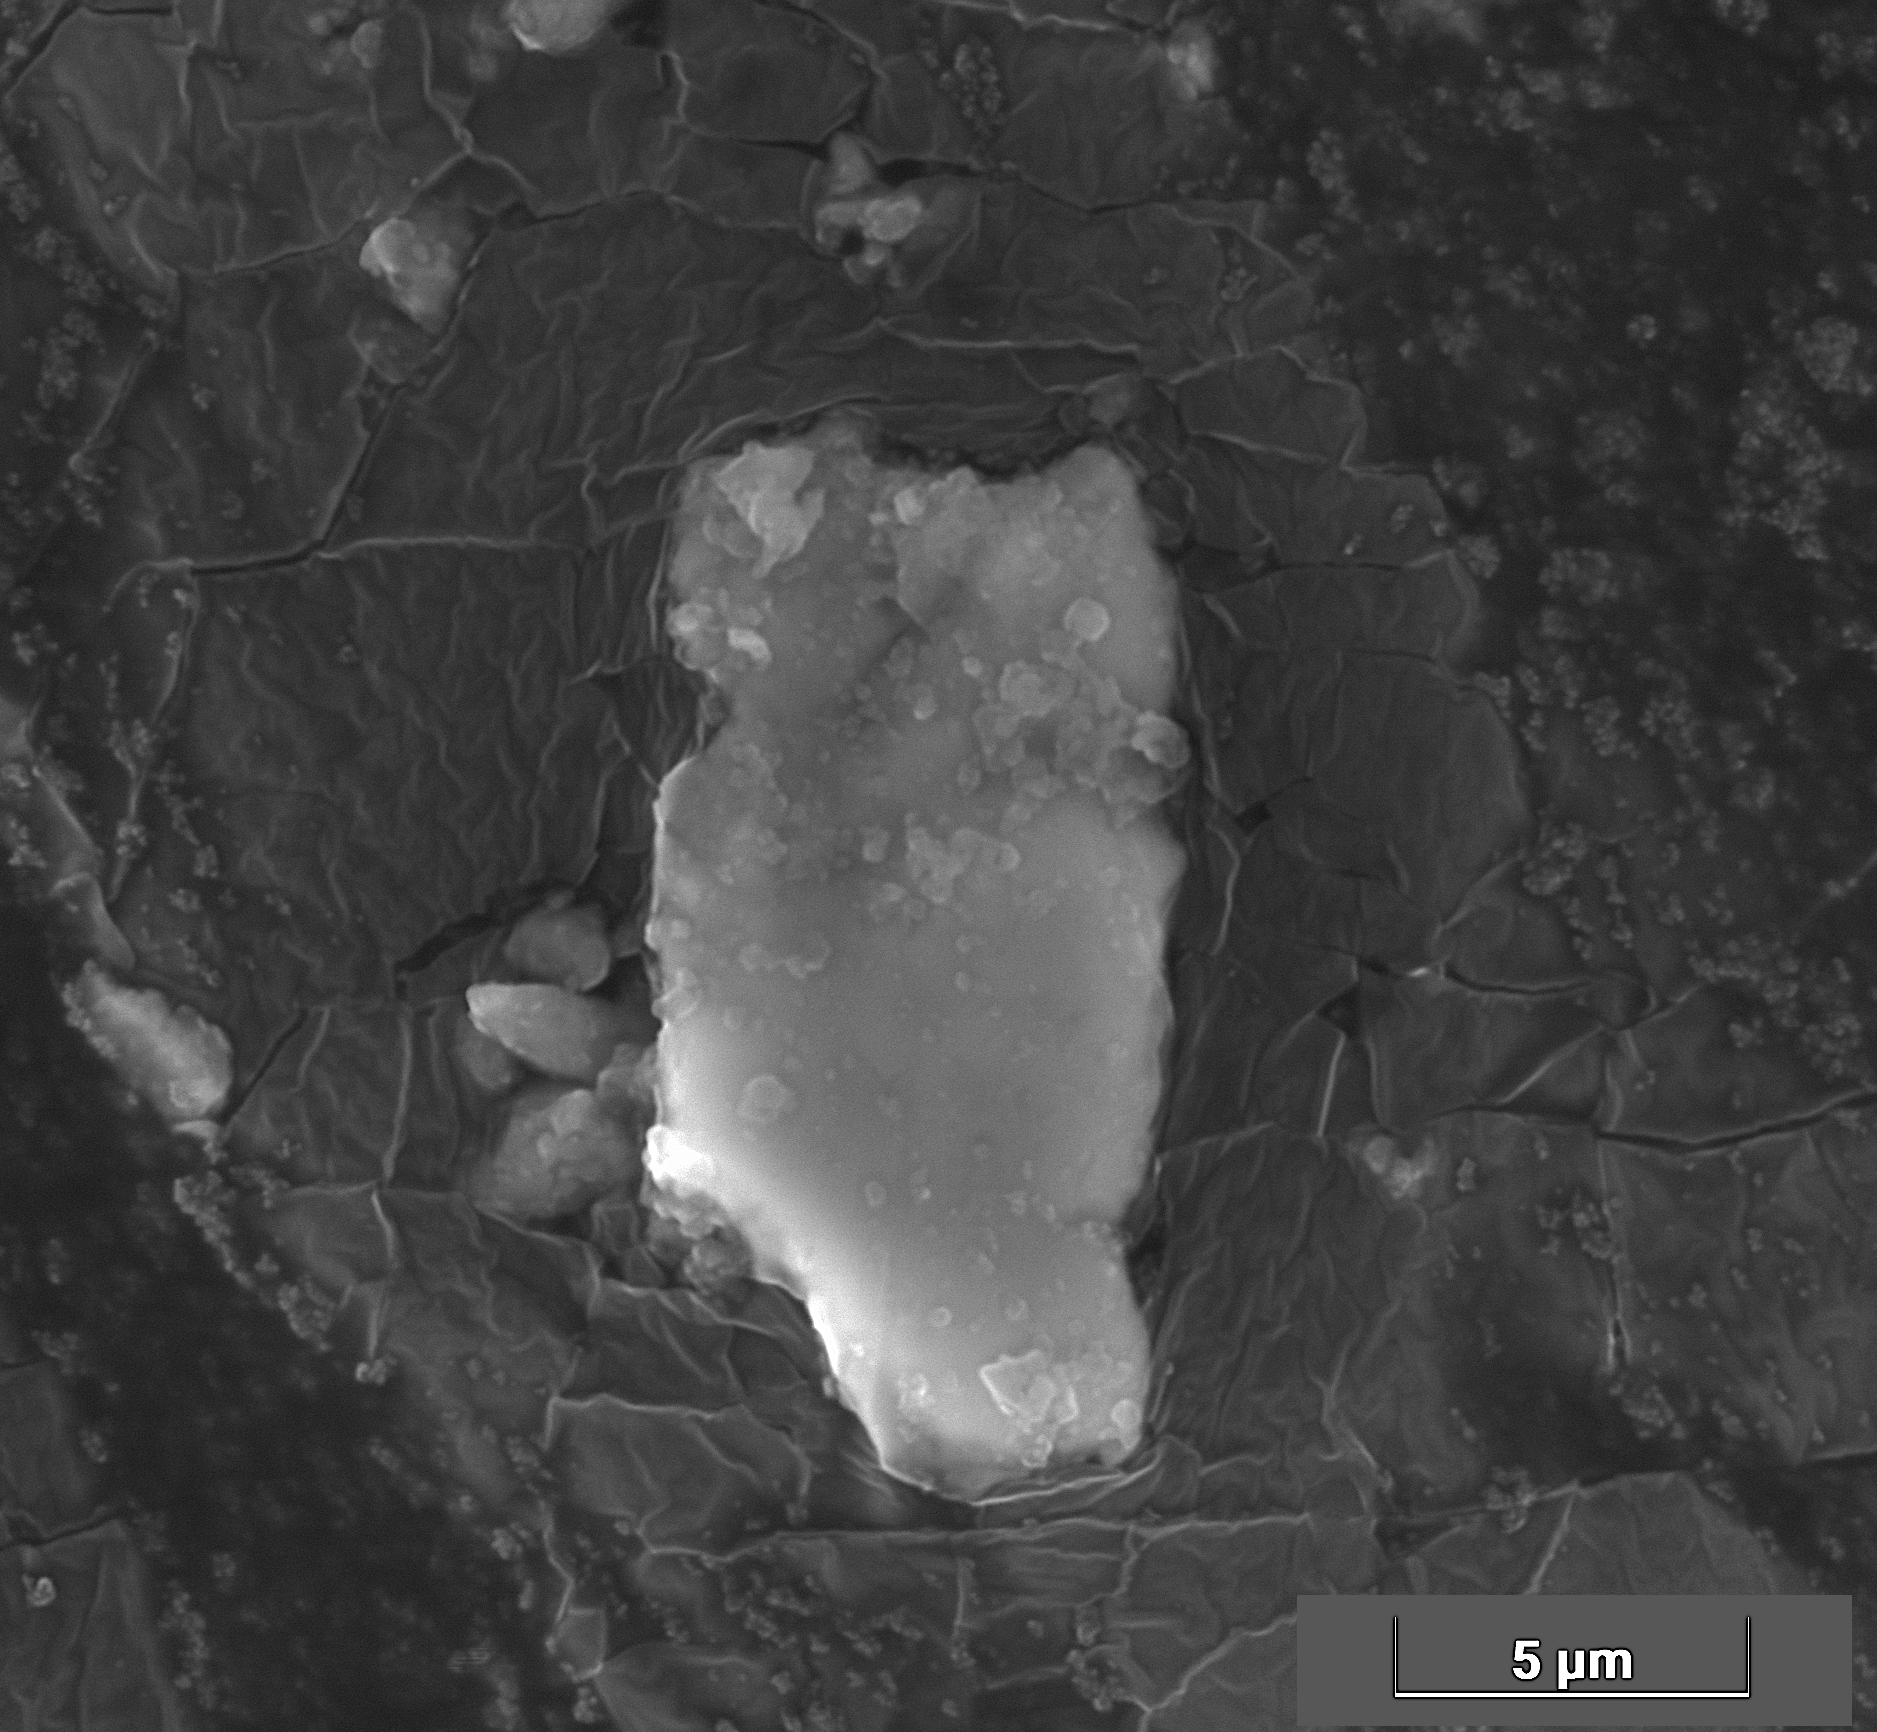
\includegraphics[width=\linewidth]{images/YPSILON POST10 lamellar.png}
		  \caption{Ypsilon Post}
		  \label{fig:Ypsilon_Post_Lamellar}
	       \end{subfigure}
\caption{Examples of lamellar shapes found in differnet samples. (a) a single lamellar particle. (b) lamellar particle with smaller ones on top. (c) on the right a lamellar particle. (d). single lamellar particle. }
	\label{fig:Lamellar}
\end{figure}




%Additionally, some particles exhibited striations, likely indicating sliding motions.






















